\documentclass[1p]{elsarticle_modified}
%\bibliographystyle{elsarticle-num}

%\usepackage[colorlinks]{hyperref}
%\usepackage{abbrmath_seonhwa} %\Abb, \Ascr, \Acal ,\Abf, \Afrak
\usepackage{amsfonts}
\usepackage{amssymb}
\usepackage{amsmath}
\usepackage{amsthm}
\usepackage{scalefnt}
\usepackage{amsbsy}
\usepackage{kotex}
\usepackage{caption}
\usepackage{subfig}
\usepackage{color}
\usepackage{graphicx}
\usepackage{xcolor} %% white, black, red, green, blue, cyan, magenta, yellow
\usepackage{float}
\usepackage{setspace}
\usepackage{hyperref}

\usepackage{tikz}
\usetikzlibrary{arrows}

\usepackage{multirow}
\usepackage{array} % fixed length table
\usepackage{hhline}

%%%%%%%%%%%%%%%%%%%%%
\makeatletter
\renewcommand*\env@matrix[1][\arraystretch]{%
	\edef\arraystretch{#1}%
	\hskip -\arraycolsep
	\let\@ifnextchar\new@ifnextchar
	\array{*\c@MaxMatrixCols c}}
\makeatother %https://tex.stackexchange.com/questions/14071/how-can-i-increase-the-line-spacing-in-a-matrix
%%%%%%%%%%%%%%%

\usepackage[normalem]{ulem}

\newcommand{\msout}[1]{\ifmmode\text{\sout{\ensuremath{#1}}}\else\sout{#1}\fi}
%SOURCE: \msout is \stkout macro in https://tex.stackexchange.com/questions/20609/strikeout-in-math-mode

\newcommand{\cancel}[1]{
	\ifmmode
	{\color{red}\msout{#1}}
	\else
	{\color{red}\sout{#1}}
	\fi
}

\newcommand{\add}[1]{
	{\color{blue}\uwave{#1}}
}

\newcommand{\replace}[2]{
	\ifmmode
	{\color{red}\msout{#1}}{\color{blue}\uwave{#2}}
	\else
	{\color{red}\sout{#1}}{\color{blue}\uwave{#2}}
	\fi
}

\newcommand{\Sol}{\mathcal{S}} %segment
\newcommand{\D}{D} %diagram
\newcommand{\A}{\mathcal{A}} %arc


%%%%%%%%%%%%%%%%%%%%%%%%%%%%%5 test

\def\sl{\operatorname{\textup{SL}}(2,\Cbb)}
\def\psl{\operatorname{\textup{PSL}}(2,\Cbb)}
\def\quan{\mkern 1mu \triangleright \mkern 1mu}

\theoremstyle{definition}
\newtheorem{thm}{Theorem}[section]
\newtheorem{prop}[thm]{Proposition}
\newtheorem{lem}[thm]{Lemma}
\newtheorem{ques}[thm]{Question}
\newtheorem{cor}[thm]{Corollary}
\newtheorem{defn}[thm]{Definition}
\newtheorem{exam}[thm]{Example}
\newtheorem{rmk}[thm]{Remark}
\newtheorem{alg}[thm]{Algorithm}

\newcommand{\I}{\sqrt{-1}}
\begin{document}

%\begin{frontmatter}
%
%\title{Boundary parabolic representations of knots up to 8 crossings}
%
%%% Group authors per affiliation:
%\author{Yunhi Cho} 
%\address{Department of Mathematics, University of Seoul, Seoul, Korea}
%\ead{yhcho@uos.ac.kr}
%
%
%\author{Seonhwa Kim} %\fnref{s_kim}}
%\address{Center for Geometry and Physics, Institute for Basic Science, Pohang, 37673, Korea}
%\ead{ryeona17@ibs.re.kr}
%
%\author{Hyuk Kim}
%\address{Department of Mathematical Sciences, Seoul National University, Seoul 08826, Korea}
%\ead{hyukkim@snu.ac.kr}
%
%\author{Seokbeom Yoon}
%\address{Department of Mathematical Sciences, Seoul National University, Seoul, 08826,  Korea}
%\ead{sbyoon15@snu.ac.kr}
%
%\begin{abstract}
%We find all boundary parabolic representation of knots up to 8 crossings.
%
%\end{abstract}
%\begin{keyword}
%    \MSC[2010] 57M25 
%\end{keyword}
%
%\end{frontmatter}

%\linenumbers
%\tableofcontents
%
\newcommand\colored[1]{\textcolor{white}{\rule[-0.35ex]{0.8em}{1.4ex}}\kern-0.8em\color{red} #1}%
%\newcommand\colored[1]{\textcolor{white}{ #1}\kern-2.17ex	\textcolor{white}{ #1}\kern-1.81ex	\textcolor{white}{ #1}\kern-2.15ex\color{red}#1	}

{\Large $\underline{12a_{1078}~(K12a_{1078})}$}

\setlength{\tabcolsep}{10pt}
\renewcommand{\arraystretch}{1.6}
\vspace{1cm}\begin{tabular}{m{100pt}>{\centering\arraybackslash}m{274pt}}
\multirow{5}{120pt}{
	\centering
	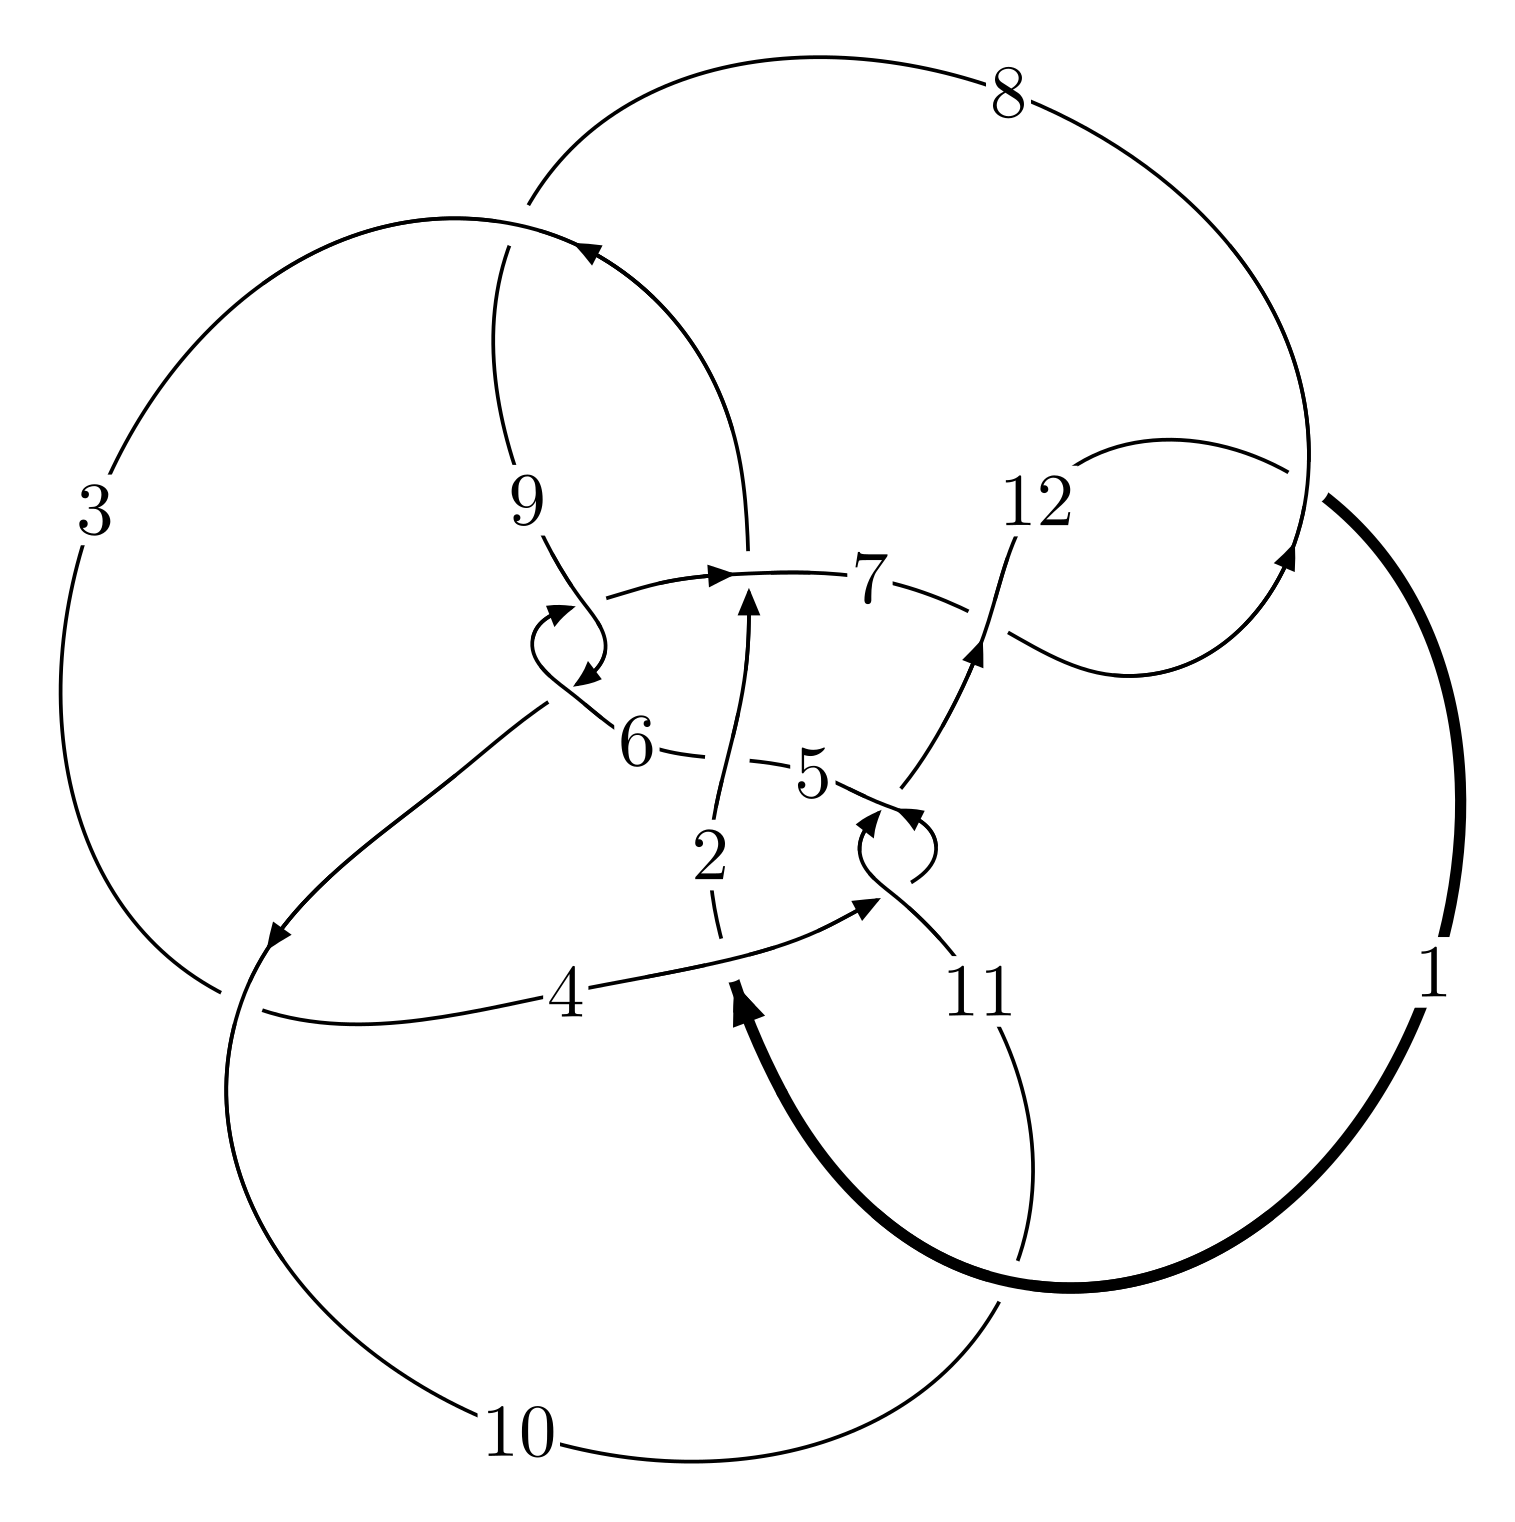
\includegraphics[width=112pt]{../../../GIT/diagram.site/Diagrams/png/1879_12a_1078.png}\\
\ \ \ A knot diagram\footnotemark}&
\allowdisplaybreaks
\textbf{Linearized knot diagam} \\
\cline{2-2}
 &
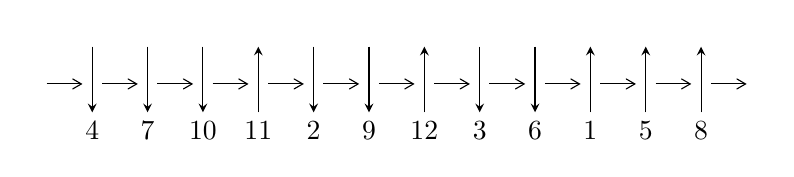
\begin{tikzpicture}[x=20pt, y=17pt]
	% nodes
	\node (C0) at (0, 0) {};
	\node (C1) at (1, 0) {};
	\node (C1U) at (1, +1) {};
	\node (C1D) at (1, -1) {4};

	\node (C2) at (2, 0) {};
	\node (C2U) at (2, +1) {};
	\node (C2D) at (2, -1) {7};

	\node (C3) at (3, 0) {};
	\node (C3U) at (3, +1) {};
	\node (C3D) at (3, -1) {10};

	\node (C4) at (4, 0) {};
	\node (C4U) at (4, +1) {};
	\node (C4D) at (4, -1) {11};

	\node (C5) at (5, 0) {};
	\node (C5U) at (5, +1) {};
	\node (C5D) at (5, -1) {2};

	\node (C6) at (6, 0) {};
	\node (C6U) at (6, +1) {};
	\node (C6D) at (6, -1) {9};

	\node (C7) at (7, 0) {};
	\node (C7U) at (7, +1) {};
	\node (C7D) at (7, -1) {12};

	\node (C8) at (8, 0) {};
	\node (C8U) at (8, +1) {};
	\node (C8D) at (8, -1) {3};

	\node (C9) at (9, 0) {};
	\node (C9U) at (9, +1) {};
	\node (C9D) at (9, -1) {6};

	\node (C10) at (10, 0) {};
	\node (C10U) at (10, +1) {};
	\node (C10D) at (10, -1) {1};

	\node (C11) at (11, 0) {};
	\node (C11U) at (11, +1) {};
	\node (C11D) at (11, -1) {5};

	\node (C12) at (12, 0) {};
	\node (C12U) at (12, +1) {};
	\node (C12D) at (12, -1) {8};
	\node (C13) at (13, 0) {};

	% arrows
	\draw[->,>={angle 60}]
	(C0) edge (C1) (C1) edge (C2) (C2) edge (C3) (C3) edge (C4) (C4) edge (C5) (C5) edge (C6) (C6) edge (C7) (C7) edge (C8) (C8) edge (C9) (C9) edge (C10) (C10) edge (C11) (C11) edge (C12) (C12) edge (C13) ;	\draw[->,>=stealth]
	(C1U) edge (C1D) (C2U) edge (C2D) (C3U) edge (C3D) (C4D) edge (C4U) (C5U) edge (C5D) (C6U) edge (C6D) (C7D) edge (C7U) (C8U) edge (C8D) (C9U) edge (C9D) (C10D) edge (C10U) (C11D) edge (C11U) (C12D) edge (C12U) ;
	\end{tikzpicture} \\
\hhline{~~} \\& 
\textbf{Solving Sequence} \\ \cline{2-2} 
 &
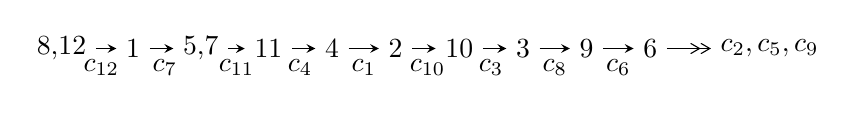
\begin{tikzpicture}[x=23pt, y=7pt]
	% node
	\node (A0) at (-1/8, 0) {8,12};
	\node (A1) at (1, 0) {1};
	\node (A2) at (33/16, 0) {5,7};
	\node (A3) at (25/8, 0) {11};
	\node (A4) at (33/8, 0) {4};
	\node (A5) at (41/8, 0) {2};
	\node (A6) at (49/8, 0) {10};
	\node (A7) at (57/8, 0) {3};
	\node (A8) at (65/8, 0) {9};
	\node (A9) at (73/8, 0) {6};
	\node (C1) at (1/2, -1) {$c_{12}$};
	\node (C2) at (3/2, -1) {$c_{7}$};
	\node (C3) at (21/8, -1) {$c_{11}$};
	\node (C4) at (29/8, -1) {$c_{4}$};
	\node (C5) at (37/8, -1) {$c_{1}$};
	\node (C6) at (45/8, -1) {$c_{10}$};
	\node (C7) at (53/8, -1) {$c_{3}$};
	\node (C8) at (61/8, -1) {$c_{8}$};
	\node (C9) at (69/8, -1) {$c_{6}$};
	\node (A10) at (11, 0) {$c_{2},c_{5},c_{9}$};

	% edge
	\draw[->,>=stealth]	
	(A0) edge (A1) (A1) edge (A2) (A2) edge (A3) (A3) edge (A4) (A4) edge (A5) (A5) edge (A6) (A6) edge (A7) (A7) edge (A8) (A8) edge (A9) ;
	\draw[->>,>={angle 60}]	
	(A9) edge (A10);
\end{tikzpicture} \\ 

\end{tabular} \\

\footnotetext{
The image of knot diagram is generated by the software ``\textbf{Draw programme}" developed by Andrew Bartholomew(\url{http://www.layer8.co.uk/maths/draw/index.htm\#Running-draw}), where we modified some parts for our purpose(\url{https://github.com/CATsTAILs/LinksPainter}).
}\phantom \\ \newline 
\centering \textbf{Ideals for irreducible components\footnotemark of $X_{\text{par}}$} 
 
\begin{align*}
I^u_{1}&=\langle 
-1.42254\times10^{1026} u^{182}-1.43895\times10^{1026} u^{181}+\cdots+2.00299\times10^{1023} b+6.70498\times10^{1025},\\
\phantom{I^u_{1}}&\phantom{= \langle  }-2.27742\times10^{1027} u^{182}-2.16805\times10^{1027} u^{181}+\cdots+2.00299\times10^{1023} a+1.25093\times10^{1027},\\
\phantom{I^u_{1}}&\phantom{= \langle  }4 u^{183}+2 u^{182}+\cdots-2 u+1\rangle \\
I^u_{2}&=\langle 
3.84908\times10^{38} u^{44}-8.37838\times10^{37} u^{43}+\cdots+2.17731\times10^{35} b-1.13314\times10^{38},\\
\phantom{I^u_{2}}&\phantom{= \langle  }5.31620\times10^{38} u^{44}-2.05529\times10^{38} u^{43}+\cdots+2.17731\times10^{35} a-1.03891\times10^{38},\;4 u^{45}-2 u^{44}+\cdots-3 u+1\rangle \\
\\
\end{align*}
\raggedright * 2 irreducible components of $\dim_{\mathbb{C}}=0$, with total 228 representations.\\
\footnotetext{All coefficients of polynomials are rational numbers. But the coefficients are sometimes approximated in decimal forms when there is not enough margin.}
\newpage
\renewcommand{\arraystretch}{1}
\centering \section*{I. $I^u_{1}= \langle -1.42\times10^{1026} u^{182}-1.44\times10^{1026} u^{181}+\cdots+2.00\times10^{1023} b+6.70\times10^{1025},\;-2.28\times10^{1027} u^{182}-2.17\times10^{1027} u^{181}+\cdots+2.00\times10^{1023} a+1.25\times10^{1027},\;4 u^{183}+2 u^{182}+\cdots-2 u+1 \rangle$}
\flushleft \textbf{(i) Arc colorings}\\
\begin{tabular}{m{7pt} m{180pt} m{7pt} m{180pt} }
\flushright $a_{8}=$&$\begin{pmatrix}0\\u\end{pmatrix}$ \\
\flushright $a_{12}=$&$\begin{pmatrix}1\\0\end{pmatrix}$ \\
\flushright $a_{1}=$&$\begin{pmatrix}1\\- u^2\end{pmatrix}$ \\
\flushright $a_{5}=$&$\begin{pmatrix}11370.1 u^{182}+10824.1 u^{181}+\cdots-1274.29 u-6245.32\\710.207 u^{182}+718.400 u^{181}+\cdots+45.9882 u-334.749\end{pmatrix}$ \\
\flushright $a_{7}=$&$\begin{pmatrix}- u\\u\end{pmatrix}$ \\
\flushright $a_{11}=$&$\begin{pmatrix}9952.46 u^{182}+9437.37 u^{181}+\cdots-1208.38 u-5503.48\\2069.74 u^{182}+2066.80 u^{181}+\cdots+22.0905 u-1020.16\end{pmatrix}$ \\
\flushright $a_{4}=$&$\begin{pmatrix}3805.30 u^{182}+3725.93 u^{181}+\cdots-166.903 u-1982.81\\-3719.84 u^{182}-3655.64 u^{181}+\cdots+148.962 u+1917.08\end{pmatrix}$ \\
\flushright $a_{2}=$&$\begin{pmatrix}-5989.26 u^{182}-5778.96 u^{181}+\cdots+488.940 u+3208.35\\558.228 u^{182}+428.115 u^{181}+\cdots-286.701 u-435.982\end{pmatrix}$ \\
\flushright $a_{10}=$&$\begin{pmatrix}5881.98 u^{182}+5475.97 u^{181}+\cdots-972.925 u-3368.03\\2981.75 u^{182}+2954.78 u^{181}+\cdots-32.4516 u-1501.70\end{pmatrix}$ \\
\flushright $a_{3}=$&$\begin{pmatrix}-4703.80 u^{182}-4514.72 u^{181}+\cdots+448.847 u+2549.52\\-727.237 u^{182}-836.129 u^{181}+\cdots-246.608 u+222.850\end{pmatrix}$ \\
\flushright $a_{9}=$&$\begin{pmatrix}10291.8 u^{182}+9908.12 u^{181}+\cdots-861.800 u-5561.15\\-584.062 u^{182}-424.879 u^{181}+\cdots+411.316 u+466.074\end{pmatrix}$ \\
\flushright $a_{6}=$&$\begin{pmatrix}-12319.2 u^{182}-12117.3 u^{181}+\cdots+361.928 u+6357.71\\11019.1 u^{182}+10663.0 u^{181}+\cdots-782.092 u-5881.84\end{pmatrix}$\\&\end{tabular}
\flushleft \textbf{(ii) Obstruction class $= -1$}\\~\\
\flushleft \textbf{(iii) Cusp Shapes $= -38193.2 u^{182}-36262.8 u^{181}+\cdots+4490.93 u+21122.6$}\\~\\
\newpage\renewcommand{\arraystretch}{1}
\flushleft \textbf{(iv) u-Polynomials at the component}\newline \\
\begin{tabular}{m{50pt}|m{274pt}}
Crossings & \hspace{64pt}u-Polynomials at each crossing \\
\hline $$\begin{aligned}c_{1}\end{aligned}$$&$\begin{aligned}
&16(16 u^{183}+252 u^{182}+\cdots+449 u-17)
\end{aligned}$\\
\hline $$\begin{aligned}c_{2}\end{aligned}$$&$\begin{aligned}
&4(4 u^{183}-14 u^{182}+\cdots+864065 u-160229)
\end{aligned}$\\
\hline $$\begin{aligned}c_{3}\end{aligned}$$&$\begin{aligned}
&u^{183}-3 u^{182}+\cdots+285506 u-6964
\end{aligned}$\\
\hline $$\begin{aligned}c_{4},c_{11}\end{aligned}$$&$\begin{aligned}
&u^{183}+5 u^{182}+\cdots+1386431 u+62039
\end{aligned}$\\
\hline $$\begin{aligned}c_{5}\end{aligned}$$&$\begin{aligned}
&u^{183}-4 u^{182}+\cdots-17118874 u-3362836
\end{aligned}$\\
\hline $$\begin{aligned}c_{6},c_{9}\end{aligned}$$&$\begin{aligned}
&u^{183}-8 u^{182}+\cdots-9204 u+773
\end{aligned}$\\
\hline $$\begin{aligned}c_{7},c_{12}\end{aligned}$$&$\begin{aligned}
&4(4 u^{183}-2 u^{182}+\cdots-2 u-1)
\end{aligned}$\\
\hline $$\begin{aligned}c_{8}\end{aligned}$$&$\begin{aligned}
&4(4 u^{183}-2 u^{182}+\cdots+4507202 u-289523)
\end{aligned}$\\
\hline $$\begin{aligned}c_{10}\end{aligned}$$&$\begin{aligned}
&u^{183}+6 u^{182}+\cdots+5277708 u+199568
\end{aligned}$\\
\hline
\end{tabular}\\~\\
\newpage\renewcommand{\arraystretch}{1}
\flushleft \textbf{(v) Riley Polynomials at the component}\newline \\
\begin{tabular}{m{50pt}|m{274pt}}
Crossings & \hspace{64pt}Riley Polynomials at each crossing \\
\hline $$\begin{aligned}c_{1}\end{aligned}$$&$\begin{aligned}
&256(256 y^{183}-2416 y^{182}+\cdots-5697 y-289)
\end{aligned}$\\
\hline $$\begin{aligned}c_{2}\end{aligned}$$&$\begin{aligned}
&16(16 y^{183}+404 y^{182}+\cdots+7.51074\times10^{11} y-2.56733\times10^{10})
\end{aligned}$\\
\hline $$\begin{aligned}c_{3}\end{aligned}$$&$\begin{aligned}
&y^{183}-55 y^{182}+\cdots+3956764060 y-48497296
\end{aligned}$\\
\hline $$\begin{aligned}c_{4},c_{11}\end{aligned}$$&$\begin{aligned}
&y^{183}-121 y^{182}+\cdots+995844174085 y-3848837521
\end{aligned}$\\
\hline $$\begin{aligned}c_{5}\end{aligned}$$&$\begin{aligned}
&y^{183}-20 y^{182}+\cdots+1169699756063260 y-11308665962896
\end{aligned}$\\
\hline $$\begin{aligned}c_{6},c_{9}\end{aligned}$$&$\begin{aligned}
&y^{183}+110 y^{182}+\cdots-36021254 y-597529
\end{aligned}$\\
\hline $$\begin{aligned}c_{7},c_{12}\end{aligned}$$&$\begin{aligned}
&16(16 y^{183}-1564 y^{182}+\cdots+82 y-1)
\end{aligned}$\\
\hline $$\begin{aligned}c_{8}\end{aligned}$$&$\begin{aligned}
&16(16 y^{183}+196 y^{182}+\cdots+3.04473\times10^{12} y-8.38236\times10^{10})
\end{aligned}$\\
\hline $$\begin{aligned}c_{10}\end{aligned}$$&$\begin{aligned}
&y^{183}-18 y^{182}+\cdots+2408586039216 y-39827386624
\end{aligned}$\\
\hline
\end{tabular}\\~\\
\newpage\flushleft \textbf{(vi) Complex Volumes and Cusp Shapes}
$$\begin{array}{c|c|c}  
\text{Solutions to }I^u_{1}& \I (\text{vol} + \sqrt{-1}CS) & \text{Cusp shape}\\
 \hline 
\begin{aligned}
u &= -0.435994 + 0.892598 I \\
a &= \phantom{-}0.844089 + 0.425621 I \\
b &= \phantom{-}1.196650 + 0.717109 I\end{aligned}
 & \phantom{-}2.66114 - 4.14393 I & \phantom{-0.000000 } 0 \\ \hline\begin{aligned}
u &= -0.435994 - 0.892598 I \\
a &= \phantom{-}0.844089 - 0.425621 I \\
b &= \phantom{-}1.196650 - 0.717109 I\end{aligned}
 & \phantom{-}2.66114 + 4.14393 I & \phantom{-0.000000 } 0 \\ \hline\begin{aligned}
u &= -0.299647 + 0.938486 I \\
a &= \phantom{-}0.725434 + 0.712589 I \\
b &= -0.019019 + 0.975825 I\end{aligned}
 & -0.93979 + 9.22059 I & \phantom{-0.000000 } 0 \\ \hline\begin{aligned}
u &= -0.299647 - 0.938486 I \\
a &= \phantom{-}0.725434 - 0.712589 I \\
b &= -0.019019 - 0.975825 I\end{aligned}
 & -0.93979 - 9.22059 I & \phantom{-0.000000 } 0 \\ \hline\begin{aligned}
u &= -0.179097 + 0.961498 I \\
a &= \phantom{-}0.979299 + 0.643036 I \\
b &= -0.012177 + 0.515658 I\end{aligned}
 & -1.03964 - 4.24096 I & \phantom{-0.000000 } 0 \\ \hline\begin{aligned}
u &= -0.179097 - 0.961498 I \\
a &= \phantom{-}0.979299 - 0.643036 I \\
b &= -0.012177 - 0.515658 I\end{aligned}
 & -1.03964 + 4.24096 I & \phantom{-0.000000 } 0 \\ \hline\begin{aligned}
u &= -0.968063 + 0.136793 I \\
a &= \phantom{-}1.124980 + 0.344421 I \\
b &= -0.450543 + 0.406317 I\end{aligned}
 & \phantom{-}1.60840 - 1.88368 I & \phantom{-0.000000 } 0 \\ \hline\begin{aligned}
u &= -0.968063 - 0.136793 I \\
a &= \phantom{-}1.124980 - 0.344421 I \\
b &= -0.450543 - 0.406317 I\end{aligned}
 & \phantom{-}1.60840 + 1.88368 I & \phantom{-0.000000 } 0 \\ \hline\begin{aligned}
u &= -0.791124 + 0.673148 I \\
a &= \phantom{-}0.377369 + 0.292424 I \\
b &= -0.893997 - 0.018281 I\end{aligned}
 & \phantom{-}1.37483 - 0.55344 I & \phantom{-0.000000 } 0 \\ \hline\begin{aligned}
u &= -0.791124 - 0.673148 I \\
a &= \phantom{-}0.377369 - 0.292424 I \\
b &= -0.893997 + 0.018281 I\end{aligned}
 & \phantom{-}1.37483 + 0.55344 I & \phantom{-0.000000 } 0\\
 \hline 
 \end{array}$$\newpage$$\begin{array}{c|c|c}  
\text{Solutions to }I^u_{1}& \I (\text{vol} + \sqrt{-1}CS) & \text{Cusp shape}\\
 \hline 
\begin{aligned}
u &= -0.927068 + 0.493900 I \\
a &= -0.081388 + 0.179395 I \\
b &= -0.730734 - 0.088837 I\end{aligned}
 & \phantom{-}1.27870 - 0.70102 I & \phantom{-0.000000 } 0 \\ \hline\begin{aligned}
u &= -0.927068 - 0.493900 I \\
a &= -0.081388 - 0.179395 I \\
b &= -0.730734 + 0.088837 I\end{aligned}
 & \phantom{-}1.27870 + 0.70102 I & \phantom{-0.000000 } 0 \\ \hline\begin{aligned}
u &= \phantom{-}1.023140 + 0.258102 I \\
a &= \phantom{-}0.251436 + 0.899798 I \\
b &= -0.552228 + 0.156044 I\end{aligned}
 & \phantom{-}5.93378 - 2.01906 I & \phantom{-0.000000 } 0 \\ \hline\begin{aligned}
u &= \phantom{-}1.023140 - 0.258102 I \\
a &= \phantom{-}0.251436 - 0.899798 I \\
b &= -0.552228 - 0.156044 I\end{aligned}
 & \phantom{-}5.93378 + 2.01906 I & \phantom{-0.000000 } 0 \\ \hline\begin{aligned}
u &= -0.201244 + 1.044460 I \\
a &= \phantom{-}0.051901 - 0.539196 I \\
b &= \phantom{-}1.267020 - 0.259232 I\end{aligned}
 & \phantom{-}0.16638 - 3.50169 I & \phantom{-0.000000 } 0 \\ \hline\begin{aligned}
u &= -0.201244 - 1.044460 I \\
a &= \phantom{-}0.051901 + 0.539196 I \\
b &= \phantom{-}1.267020 + 0.259232 I\end{aligned}
 & \phantom{-}0.16638 + 3.50169 I & \phantom{-0.000000 } 0 \\ \hline\begin{aligned}
u &= -0.884541 + 0.301835 I \\
a &= -0.884826 + 0.843686 I \\
b &= \phantom{-}0.195765 - 1.292020 I\end{aligned}
 & -1.19560 - 1.79116 I & \phantom{-0.000000 } 0 \\ \hline\begin{aligned}
u &= -0.884541 - 0.301835 I \\
a &= -0.884826 - 0.843686 I \\
b &= \phantom{-}0.195765 + 1.292020 I\end{aligned}
 & -1.19560 + 1.79116 I & \phantom{-0.000000 } 0 \\ \hline\begin{aligned}
u &= \phantom{-}0.245347 + 1.037970 I \\
a &= -1.246090 - 0.362330 I \\
b &= \phantom{-}0.904434 + 0.036830 I\end{aligned}
 & -1.37820 + 3.10134 I & \phantom{-0.000000 } 0 \\ \hline\begin{aligned}
u &= \phantom{-}0.245347 - 1.037970 I \\
a &= -1.246090 + 0.362330 I \\
b &= \phantom{-}0.904434 - 0.036830 I\end{aligned}
 & -1.37820 - 3.10134 I & \phantom{-0.000000 } 0\\
 \hline 
 \end{array}$$\newpage$$\begin{array}{c|c|c}  
\text{Solutions to }I^u_{1}& \I (\text{vol} + \sqrt{-1}CS) & \text{Cusp shape}\\
 \hline 
\begin{aligned}
u &= \phantom{-}1.007680 + 0.351734 I \\
a &= \phantom{-}1.111550 - 0.050183 I \\
b &= -0.373220 - 0.770569 I\end{aligned}
 & \phantom{-}1.52893 + 0.67044 I & \phantom{-0.000000 } 0 \\ \hline\begin{aligned}
u &= \phantom{-}1.007680 - 0.351734 I \\
a &= \phantom{-}1.111550 + 0.050183 I \\
b &= -0.373220 + 0.770569 I\end{aligned}
 & \phantom{-}1.52893 - 0.67044 I & \phantom{-0.000000 } 0 \\ \hline\begin{aligned}
u &= \phantom{-}0.563418 + 0.923911 I \\
a &= \phantom{-}0.466978 + 0.198414 I \\
b &= -1.266650 + 0.494142 I\end{aligned}
 & \phantom{-}5.96882 - 2.77936 I & \phantom{-0.000000 } 0 \\ \hline\begin{aligned}
u &= \phantom{-}0.563418 - 0.923911 I \\
a &= \phantom{-}0.466978 - 0.198414 I \\
b &= -1.266650 - 0.494142 I\end{aligned}
 & \phantom{-}5.96882 + 2.77936 I & \phantom{-0.000000 } 0 \\ \hline\begin{aligned}
u &= \phantom{-}0.318840 + 1.038110 I \\
a &= \phantom{-}0.716550 - 0.753529 I \\
b &= \phantom{-}0.057847 - 0.951617 I\end{aligned}
 & -4.79655 - 2.89380 I & \phantom{-0.000000 } 0 \\ \hline\begin{aligned}
u &= \phantom{-}0.318840 - 1.038110 I \\
a &= \phantom{-}0.716550 + 0.753529 I \\
b &= \phantom{-}0.057847 + 0.951617 I\end{aligned}
 & -4.79655 + 2.89380 I & \phantom{-0.000000 } 0 \\ \hline\begin{aligned}
u &= -0.691890 + 0.588159 I \\
a &= \phantom{-}0.613586 + 0.354824 I \\
b &= -0.298548 - 0.446290 I\end{aligned}
 & \phantom{-}1.80572 + 3.17497 I & \phantom{-0.000000 } 0 \\ \hline\begin{aligned}
u &= -0.691890 - 0.588159 I \\
a &= \phantom{-}0.613586 - 0.354824 I \\
b &= -0.298548 + 0.446290 I\end{aligned}
 & \phantom{-}1.80572 - 3.17497 I & \phantom{-0.000000 } 0 \\ \hline\begin{aligned}
u &= -1.077300 + 0.189760 I \\
a &= \phantom{-}0.203809 + 0.380584 I \\
b &= -0.789435 - 1.019960 I\end{aligned}
 & \phantom{-}1.54583 - 0.00514 I & \phantom{-0.000000 } 0 \\ \hline\begin{aligned}
u &= -1.077300 - 0.189760 I \\
a &= \phantom{-}0.203809 - 0.380584 I \\
b &= -0.789435 + 1.019960 I\end{aligned}
 & \phantom{-}1.54583 + 0.00514 I & \phantom{-0.000000 } 0\\
 \hline 
 \end{array}$$\newpage$$\begin{array}{c|c|c}  
\text{Solutions to }I^u_{1}& \I (\text{vol} + \sqrt{-1}CS) & \text{Cusp shape}\\
 \hline 
\begin{aligned}
u &= \phantom{-}0.811749 + 0.390367 I \\
a &= -0.906879 - 0.564551 I \\
b &= \phantom{-}0.402641 + 0.931175 I\end{aligned}
 & -1.10562 + 5.08781 I & \phantom{-0.000000 } 0 \\ \hline\begin{aligned}
u &= \phantom{-}0.811749 - 0.390367 I \\
a &= -0.906879 + 0.564551 I \\
b &= \phantom{-}0.402641 - 0.931175 I\end{aligned}
 & -1.10562 - 5.08781 I & \phantom{-0.000000 } 0 \\ \hline\begin{aligned}
u &= -1.014490 + 0.423498 I \\
a &= -0.578315 + 0.697424 I \\
b &= -0.360178 - 0.895200 I\end{aligned}
 & \phantom{-}1.17751 - 5.41890 I & \phantom{-0.000000 } 0 \\ \hline\begin{aligned}
u &= -1.014490 - 0.423498 I \\
a &= -0.578315 - 0.697424 I \\
b &= -0.360178 + 0.895200 I\end{aligned}
 & \phantom{-}1.17751 + 5.41890 I & \phantom{-0.000000 } 0 \\ \hline\begin{aligned}
u &= \phantom{-}0.996685 + 0.488016 I \\
a &= -0.494469 - 0.641126 I \\
b &= -0.386486 + 0.577659 I\end{aligned}
 & -0.01244 + 3.89579 I & \phantom{-0.000000 } 0 \\ \hline\begin{aligned}
u &= \phantom{-}0.996685 - 0.488016 I \\
a &= -0.494469 + 0.641126 I \\
b &= -0.386486 - 0.577659 I\end{aligned}
 & -0.01244 - 3.89579 I & \phantom{-0.000000 } 0 \\ \hline\begin{aligned}
u &= \phantom{-}1.032780 + 0.420974 I \\
a &= \phantom{-}1.129910 + 0.411137 I \\
b &= -1.199630 + 0.471004 I\end{aligned}
 & \phantom{-}5.41047 - 3.94815 I & \phantom{-0.000000 } 0 \\ \hline\begin{aligned}
u &= \phantom{-}1.032780 - 0.420974 I \\
a &= \phantom{-}1.129910 - 0.411137 I \\
b &= -1.199630 - 0.471004 I\end{aligned}
 & \phantom{-}5.41047 + 3.94815 I & \phantom{-0.000000 } 0 \\ \hline\begin{aligned}
u &= \phantom{-}1.101950 + 0.288670 I \\
a &= -0.288416 - 0.505335 I \\
b &= -0.563293 + 1.116030 I\end{aligned}
 & \phantom{-}6.33450 + 4.14277 I & \phantom{-0.000000 } 0 \\ \hline\begin{aligned}
u &= \phantom{-}1.101950 - 0.288670 I \\
a &= -0.288416 + 0.505335 I \\
b &= -0.563293 - 1.116030 I\end{aligned}
 & \phantom{-}6.33450 - 4.14277 I & \phantom{-0.000000 } 0\\
 \hline 
 \end{array}$$\newpage$$\begin{array}{c|c|c}  
\text{Solutions to }I^u_{1}& \I (\text{vol} + \sqrt{-1}CS) & \text{Cusp shape}\\
 \hline 
\begin{aligned}
u &= -0.834096 + 0.109112 I \\
a &= -3.07979 - 0.00775 I \\
b &= \phantom{-}1.43386 - 0.77030 I\end{aligned}
 & \phantom{-}0.57305 - 1.40697 I & \phantom{-0.000000 } 0 \\ \hline\begin{aligned}
u &= -0.834096 - 0.109112 I \\
a &= -3.07979 + 0.00775 I \\
b &= \phantom{-}1.43386 + 0.77030 I\end{aligned}
 & \phantom{-}0.57305 + 1.40697 I & \phantom{-0.000000 } 0 \\ \hline\begin{aligned}
u &= \phantom{-}0.836413 + 0.062418 I \\
a &= -2.99172 + 0.61737 I \\
b &= \phantom{-}1.057480 + 0.593839 I\end{aligned}
 & \phantom{-}4.69954 - 2.73836 I & \phantom{-0.000000 } 0 \\ \hline\begin{aligned}
u &= \phantom{-}0.836413 - 0.062418 I \\
a &= -2.99172 - 0.61737 I \\
b &= \phantom{-}1.057480 - 0.593839 I\end{aligned}
 & \phantom{-}4.69954 + 2.73836 I & \phantom{-0.000000 } 0 \\ \hline\begin{aligned}
u &= \phantom{-}0.630957 + 0.550000 I \\
a &= -0.732526 - 0.182055 I \\
b &= \phantom{-}0.749114 + 0.488562 I\end{aligned}
 & -0.58612 + 4.96450 I & \phantom{-0.000000 } 0 \\ \hline\begin{aligned}
u &= \phantom{-}0.630957 - 0.550000 I \\
a &= -0.732526 + 0.182055 I \\
b &= \phantom{-}0.749114 - 0.488562 I\end{aligned}
 & -0.58612 - 4.96450 I & \phantom{-0.000000 } 0 \\ \hline\begin{aligned}
u &= \phantom{-}0.995413 + 0.604085 I \\
a &= -0.448626 - 0.325962 I \\
b &= \phantom{-}0.0927846 - 0.0130873 I\end{aligned}
 & -0.24551 + 4.75126 I & \phantom{-0.000000 } 0 \\ \hline\begin{aligned}
u &= \phantom{-}0.995413 - 0.604085 I \\
a &= -0.448626 + 0.325962 I \\
b &= \phantom{-}0.0927846 + 0.0130873 I\end{aligned}
 & -0.24551 - 4.75126 I & \phantom{-0.000000 } 0 \\ \hline\begin{aligned}
u &= \phantom{-}1.057020 + 0.521499 I \\
a &= -0.243692 - 1.314180 I \\
b &= -0.757740 - 0.296570 I\end{aligned}
 & -0.26634 + 5.32691 I & \phantom{-0.000000 } 0 \\ \hline\begin{aligned}
u &= \phantom{-}1.057020 - 0.521499 I \\
a &= -0.243692 + 1.314180 I \\
b &= -0.757740 + 0.296570 I\end{aligned}
 & -0.26634 - 5.32691 I & \phantom{-0.000000 } 0\\
 \hline 
 \end{array}$$\newpage$$\begin{array}{c|c|c}  
\text{Solutions to }I^u_{1}& \I (\text{vol} + \sqrt{-1}CS) & \text{Cusp shape}\\
 \hline 
\begin{aligned}
u &= -0.774385 + 0.242007 I \\
a &= -0.937885 + 0.332567 I \\
b &= \phantom{-}0.443642 - 1.150540 I\end{aligned}
 & -1.62107 - 0.90334 I & \phantom{-0.000000 } 0 \\ \hline\begin{aligned}
u &= -0.774385 - 0.242007 I \\
a &= -0.937885 - 0.332567 I \\
b &= \phantom{-}0.443642 + 1.150540 I\end{aligned}
 & -1.62107 + 0.90334 I & \phantom{-0.000000 } 0 \\ \hline\begin{aligned}
u &= \phantom{-}1.154430 + 0.337643 I \\
a &= -0.182258 + 0.963816 I \\
b &= -0.612179 + 0.412519 I\end{aligned}
 & \phantom{-}3.48053 + 7.86335 I & \phantom{-0.000000 } 0 \\ \hline\begin{aligned}
u &= \phantom{-}1.154430 - 0.337643 I \\
a &= -0.182258 - 0.963816 I \\
b &= -0.612179 - 0.412519 I\end{aligned}
 & \phantom{-}3.48053 - 7.86335 I & \phantom{-0.000000 } 0 \\ \hline\begin{aligned}
u &= \phantom{-}0.726929 + 0.324876 I \\
a &= -0.263271 - 0.299473 I \\
b &= \phantom{-}0.175979 + 0.973124 I\end{aligned}
 & -1.41163 - 1.73255 I & \phantom{-0.000000 } 0 \\ \hline\begin{aligned}
u &= \phantom{-}0.726929 - 0.324876 I \\
a &= -0.263271 + 0.299473 I \\
b &= \phantom{-}0.175979 - 0.973124 I\end{aligned}
 & -1.41163 + 1.73255 I & \phantom{-0.000000 } 0 \\ \hline\begin{aligned}
u &= \phantom{-}0.785385 + 0.125564 I \\
a &= -3.66711 + 0.16395 I \\
b &= \phantom{-}1.64059 + 0.38662 I\end{aligned}
 & \phantom{-}4.18115 + 6.46744 I & \phantom{-0.000000 } 0 \\ \hline\begin{aligned}
u &= \phantom{-}0.785385 - 0.125564 I \\
a &= -3.66711 - 0.16395 I \\
b &= \phantom{-}1.64059 - 0.38662 I\end{aligned}
 & \phantom{-}4.18115 - 6.46744 I & \phantom{-0.000000 } 0 \\ \hline\begin{aligned}
u &= -0.369299 + 0.700251 I \\
a &= -0.157572 + 0.892871 I \\
b &= \phantom{-}1.047660 - 0.169183 I\end{aligned}
 & \phantom{-}5.08933 - 5.93229 I & \phantom{-0.000000 } 0 \\ \hline\begin{aligned}
u &= -0.369299 - 0.700251 I \\
a &= -0.157572 - 0.892871 I \\
b &= \phantom{-}1.047660 + 0.169183 I\end{aligned}
 & \phantom{-}5.08933 + 5.93229 I & \phantom{-0.000000 } 0\\
 \hline 
 \end{array}$$\newpage$$\begin{array}{c|c|c}  
\text{Solutions to }I^u_{1}& \I (\text{vol} + \sqrt{-1}CS) & \text{Cusp shape}\\
 \hline 
\begin{aligned}
u &= -1.093420 + 0.525497 I \\
a &= \phantom{-}0.26291 + 2.03387 I \\
b &= -0.977322 + 0.284930 I\end{aligned}
 & \phantom{-}4.46992 - 10.86910 I & \phantom{-0.000000 } 0 \\ \hline\begin{aligned}
u &= -1.093420 - 0.525497 I \\
a &= \phantom{-}0.26291 - 2.03387 I \\
b &= -0.977322 - 0.284930 I\end{aligned}
 & \phantom{-}4.46992 + 10.86910 I & \phantom{-0.000000 } 0 \\ \hline\begin{aligned}
u &= \phantom{-}1.148310 + 0.401673 I \\
a &= \phantom{-}2.57107 - 0.49046 I \\
b &= -1.368470 - 0.181234 I\end{aligned}
 & \phantom{-}8.69744 + 9.16930 I & \phantom{-0.000000 } 0 \\ \hline\begin{aligned}
u &= \phantom{-}1.148310 - 0.401673 I \\
a &= \phantom{-}2.57107 + 0.49046 I \\
b &= -1.368470 + 0.181234 I\end{aligned}
 & \phantom{-}8.69744 - 9.16930 I & \phantom{-0.000000 } 0 \\ \hline\begin{aligned}
u &= -0.432954 + 0.648653 I \\
a &= \phantom{-}0.373107 - 1.005890 I \\
b &= \phantom{-}0.984194 - 0.292578 I\end{aligned}
 & \phantom{-}0.07141 - 3.72785 I & \phantom{-0.000000 } 0 \\ \hline\begin{aligned}
u &= -0.432954 - 0.648653 I \\
a &= \phantom{-}0.373107 + 1.005890 I \\
b &= \phantom{-}0.984194 + 0.292578 I\end{aligned}
 & \phantom{-}0.07141 + 3.72785 I & \phantom{-0.000000 } 0 \\ \hline\begin{aligned}
u &= -1.160210 + 0.408959 I \\
a &= \phantom{-}2.36187 + 0.87124 I \\
b &= -1.220010 + 0.432666 I\end{aligned}
 & \phantom{-}2.86398 - 7.89511 I & \phantom{-0.000000 } 0 \\ \hline\begin{aligned}
u &= -1.160210 - 0.408959 I \\
a &= \phantom{-}2.36187 - 0.87124 I \\
b &= -1.220010 - 0.432666 I\end{aligned}
 & \phantom{-}2.86398 + 7.89511 I & \phantom{-0.000000 } 0 \\ \hline\begin{aligned}
u &= \phantom{-}1.155610 + 0.425076 I \\
a &= \phantom{-}2.19095 - 1.00324 I \\
b &= -1.225060 - 0.567501 I\end{aligned}
 & \phantom{-}3.95878 + 10.87850 I & \phantom{-0.000000 } 0 \\ \hline\begin{aligned}
u &= \phantom{-}1.155610 - 0.425076 I \\
a &= \phantom{-}2.19095 + 1.00324 I \\
b &= -1.225060 + 0.567501 I\end{aligned}
 & \phantom{-}3.95878 - 10.87850 I & \phantom{-0.000000 } 0\\
 \hline 
 \end{array}$$\newpage$$\begin{array}{c|c|c}  
\text{Solutions to }I^u_{1}& \I (\text{vol} + \sqrt{-1}CS) & \text{Cusp shape}\\
 \hline 
\begin{aligned}
u &= -0.510620 + 0.568691 I \\
a &= \phantom{-}0.754085 + 0.628865 I \\
b &= -0.028269 + 0.827369 I\end{aligned}
 & \phantom{-}2.32835 - 2.09541 I & \phantom{-0.000000 } 0 \\ \hline\begin{aligned}
u &= -0.510620 - 0.568691 I \\
a &= \phantom{-}0.754085 - 0.628865 I \\
b &= -0.028269 - 0.827369 I\end{aligned}
 & \phantom{-}2.32835 + 2.09541 I & \phantom{-0.000000 } 0 \\ \hline\begin{aligned}
u &= \phantom{-}0.462933 + 0.606757 I \\
a &= \phantom{-}1.62969 - 0.29323 I \\
b &= \phantom{-}0.915285 - 0.203760 I\end{aligned}
 & -2.02037 - 0.85680 I & \phantom{-0.000000 } 0 \\ \hline\begin{aligned}
u &= \phantom{-}0.462933 - 0.606757 I \\
a &= \phantom{-}1.62969 + 0.29323 I \\
b &= \phantom{-}0.915285 + 0.203760 I\end{aligned}
 & -2.02037 + 0.85680 I & \phantom{-0.000000 } 0 \\ \hline\begin{aligned}
u &= -1.168190 + 0.406675 I \\
a &= \phantom{-}0.058099 - 0.856266 I \\
b &= -0.781953 - 0.489895 I\end{aligned}
 & -0.04935 - 1.76185 I & \phantom{-0.000000 } 0 \\ \hline\begin{aligned}
u &= -1.168190 - 0.406675 I \\
a &= \phantom{-}0.058099 + 0.856266 I \\
b &= -0.781953 + 0.489895 I\end{aligned}
 & -0.04935 + 1.76185 I & \phantom{-0.000000 } 0 \\ \hline\begin{aligned}
u &= \phantom{-}0.758589 + 0.046364 I \\
a &= -6.43651 + 0.72336 I \\
b &= \phantom{-}0.933852 - 0.056164 I\end{aligned}
 & \phantom{-}1.28344 - 6.23630 I & \phantom{-0.000000 } 0 \\ \hline\begin{aligned}
u &= \phantom{-}0.758589 - 0.046364 I \\
a &= -6.43651 - 0.72336 I \\
b &= \phantom{-}0.933852 + 0.056164 I\end{aligned}
 & \phantom{-}1.28344 + 6.23630 I & \phantom{-0.000000 } 0 \\ \hline\begin{aligned}
u &= -1.163610 + 0.435310 I \\
a &= \phantom{-}0.149422 + 0.146164 I \\
b &= -0.212104 + 0.761549 I\end{aligned}
 & \phantom{-}2.46618 - 0.66784 I & \phantom{-0.000000 } 0 \\ \hline\begin{aligned}
u &= -1.163610 - 0.435310 I \\
a &= \phantom{-}0.149422 - 0.146164 I \\
b &= -0.212104 - 0.761549 I\end{aligned}
 & \phantom{-}2.46618 + 0.66784 I & \phantom{-0.000000 } 0\\
 \hline 
 \end{array}$$\newpage$$\begin{array}{c|c|c}  
\text{Solutions to }I^u_{1}& \I (\text{vol} + \sqrt{-1}CS) & \text{Cusp shape}\\
 \hline 
\begin{aligned}
u &= -1.178250 + 0.394308 I \\
a &= \phantom{-}2.18898 + 0.55295 I \\
b &= -1.46899 + 0.47141 I\end{aligned}
 & \phantom{-}4.66947 - 10.32320 I & \phantom{-0.000000 } 0 \\ \hline\begin{aligned}
u &= -1.178250 - 0.394308 I \\
a &= \phantom{-}2.18898 - 0.55295 I \\
b &= -1.46899 - 0.47141 I\end{aligned}
 & \phantom{-}4.66947 + 10.32320 I & \phantom{-0.000000 } 0 \\ \hline\begin{aligned}
u &= -1.172400 + 0.412890 I \\
a &= \phantom{-}2.52642 + 0.93741 I \\
b &= -1.127020 + 0.253372 I\end{aligned}
 & \phantom{-}2.83838 - 6.86953 I & \phantom{-0.000000 } 0 \\ \hline\begin{aligned}
u &= -1.172400 - 0.412890 I \\
a &= \phantom{-}2.52642 - 0.93741 I \\
b &= -1.127020 - 0.253372 I\end{aligned}
 & \phantom{-}2.83838 + 6.86953 I & \phantom{-0.000000 } 0 \\ \hline\begin{aligned}
u &= \phantom{-}1.144590 + 0.515377 I \\
a &= -1.67031 + 1.08084 I \\
b &= \phantom{-}1.272430 + 0.159876 I\end{aligned}
 & \phantom{-}7.38774 + 4.06024 I & \phantom{-0.000000 } 0 \\ \hline\begin{aligned}
u &= \phantom{-}1.144590 - 0.515377 I \\
a &= -1.67031 - 1.08084 I \\
b &= \phantom{-}1.272430 - 0.159876 I\end{aligned}
 & \phantom{-}7.38774 - 4.06024 I & \phantom{-0.000000 } 0 \\ \hline\begin{aligned}
u &= \phantom{-}1.235570 + 0.245822 I \\
a &= -0.1300980 + 0.0298962 I \\
b &= -0.619384 + 0.925932 I\end{aligned}
 & \phantom{-}4.30533 - 5.68525 I & \phantom{-0.000000 } 0 \\ \hline\begin{aligned}
u &= \phantom{-}1.235570 - 0.245822 I \\
a &= -0.1300980 - 0.0298962 I \\
b &= -0.619384 - 0.925932 I\end{aligned}
 & \phantom{-}4.30533 + 5.68525 I & \phantom{-0.000000 } 0 \\ \hline\begin{aligned}
u &= \phantom{-}1.215800 + 0.338826 I \\
a &= \phantom{-}1.52422 - 0.70147 I \\
b &= -1.86632 + 0.42438 I\end{aligned}
 & \phantom{-}7.49302 + 7.56242 I & \phantom{-0.000000 } 0 \\ \hline\begin{aligned}
u &= \phantom{-}1.215800 - 0.338826 I \\
a &= \phantom{-}1.52422 + 0.70147 I \\
b &= -1.86632 - 0.42438 I\end{aligned}
 & \phantom{-}7.49302 - 7.56242 I & \phantom{-0.000000 } 0\\
 \hline 
 \end{array}$$\newpage$$\begin{array}{c|c|c}  
\text{Solutions to }I^u_{1}& \I (\text{vol} + \sqrt{-1}CS) & \text{Cusp shape}\\
 \hline 
\begin{aligned}
u &= -0.737636\phantom{ +0.000000I} \\
a &= -7.07184\phantom{ +0.000000I} \\
b &= \phantom{-}0.931905\phantom{ +0.000000I}\end{aligned}
 & -2.84479\phantom{ +0.000000I} & \phantom{-0.000000 } 0 \\ \hline\begin{aligned}
u &= -0.676019 + 0.288627 I \\
a &= \phantom{-}0.440573 + 0.006647 I \\
b &= -0.741023 + 0.217066 I\end{aligned}
 & \phantom{-}1.43722 - 0.66748 I & \phantom{-0.000000 } 0 \\ \hline\begin{aligned}
u &= -0.676019 - 0.288627 I \\
a &= \phantom{-}0.440573 - 0.006647 I \\
b &= -0.741023 - 0.217066 I\end{aligned}
 & \phantom{-}1.43722 + 0.66748 I & \phantom{-0.000000 } 0 \\ \hline\begin{aligned}
u &= \phantom{-}1.197210 + 0.409750 I \\
a &= \phantom{-}1.99292 - 0.63256 I \\
b &= -1.42122 - 0.57584 I\end{aligned}
 & \phantom{-}3.68508 + 8.18402 I & \phantom{-0.000000 } 0 \\ \hline\begin{aligned}
u &= \phantom{-}1.197210 - 0.409750 I \\
a &= \phantom{-}1.99292 + 0.63256 I \\
b &= -1.42122 + 0.57584 I\end{aligned}
 & \phantom{-}3.68508 - 8.18402 I & \phantom{-0.000000 } 0 \\ \hline\begin{aligned}
u &= -0.393752 + 0.617992 I \\
a &= \phantom{-}1.63097 + 1.01161 I \\
b &= \phantom{-}1.071630 + 0.127140 I\end{aligned}
 & \phantom{-}2.39503 + 6.32987 I & \phantom{-0.000000 } 0 \\ \hline\begin{aligned}
u &= -0.393752 - 0.617992 I \\
a &= \phantom{-}1.63097 - 1.01161 I \\
b &= \phantom{-}1.071630 - 0.127140 I\end{aligned}
 & \phantom{-}2.39503 - 6.32987 I & \phantom{-0.000000 } 0 \\ \hline\begin{aligned}
u &= \phantom{-}0.342351 + 1.225570 I \\
a &= \phantom{-}0.457285 + 0.222768 I \\
b &= -1.319170 + 0.501865 I\end{aligned}
 & \phantom{-}3.1050 - 14.5175 I & \phantom{-0.000000 } 0 \\ \hline\begin{aligned}
u &= \phantom{-}0.342351 - 1.225570 I \\
a &= \phantom{-}0.457285 - 0.222768 I \\
b &= -1.319170 - 0.501865 I\end{aligned}
 & \phantom{-}3.1050 + 14.5175 I & \phantom{-0.000000 } 0 \\ \hline\begin{aligned}
u &= -1.191490 + 0.456262 I \\
a &= -1.92949 - 0.97155 I \\
b &= \phantom{-}1.42104 - 0.27469 I\end{aligned}
 & \phantom{-}7.59045 - 4.44666 I & \phantom{-0.000000 } 0\\
 \hline 
 \end{array}$$\newpage$$\begin{array}{c|c|c}  
\text{Solutions to }I^u_{1}& \I (\text{vol} + \sqrt{-1}CS) & \text{Cusp shape}\\
 \hline 
\begin{aligned}
u &= -1.191490 - 0.456262 I \\
a &= -1.92949 + 0.97155 I \\
b &= \phantom{-}1.42104 + 0.27469 I\end{aligned}
 & \phantom{-}7.59045 + 4.44666 I & \phantom{-0.000000 } 0 \\ \hline\begin{aligned}
u &= -1.181640 + 0.481453 I \\
a &= \phantom{-}1.71341 + 1.02674 I \\
b &= -1.32595 + 0.73205 I\end{aligned}
 & \phantom{-}8.9536 - 11.1741 I & \phantom{-0.000000 } 0 \\ \hline\begin{aligned}
u &= -1.181640 - 0.481453 I \\
a &= \phantom{-}1.71341 - 1.02674 I \\
b &= -1.32595 - 0.73205 I\end{aligned}
 & \phantom{-}8.9536 + 11.1741 I & \phantom{-0.000000 } 0 \\ \hline\begin{aligned}
u &= -0.039731 + 0.713005 I \\
a &= \phantom{-}0.453123 - 0.057961 I \\
b &= -1.201940 - 0.147605 I\end{aligned}
 & \phantom{-}4.26793 + 0.11022 I & \phantom{-0.000000 } 0 \\ \hline\begin{aligned}
u &= -0.039731 - 0.713005 I \\
a &= \phantom{-}0.453123 + 0.057961 I \\
b &= -1.201940 + 0.147605 I\end{aligned}
 & \phantom{-}4.26793 - 0.11022 I & \phantom{-0.000000 } 0 \\ \hline\begin{aligned}
u &= \phantom{-}0.370607 + 0.602926 I \\
a &= \phantom{-}0.0770151 + 0.0774324 I \\
b &= \phantom{-}1.082870 + 0.431455 I\end{aligned}
 & \phantom{-}0.95207 + 6.99078 I & \phantom{-0.000000 } 0 \\ \hline\begin{aligned}
u &= \phantom{-}0.370607 - 0.602926 I \\
a &= \phantom{-}0.0770151 - 0.0774324 I \\
b &= \phantom{-}1.082870 - 0.431455 I\end{aligned}
 & \phantom{-}0.95207 - 6.99078 I & \phantom{-0.000000 } 0 \\ \hline\begin{aligned}
u &= \phantom{-}1.209280 + 0.456420 I \\
a &= \phantom{-}1.31982 - 0.66160 I \\
b &= -1.44690 + 0.37540 I\end{aligned}
 & \phantom{-}9.15948 - 2.52691 I & \phantom{-0.000000 } 0 \\ \hline\begin{aligned}
u &= \phantom{-}1.209280 - 0.456420 I \\
a &= \phantom{-}1.31982 + 0.66160 I \\
b &= -1.44690 - 0.37540 I\end{aligned}
 & \phantom{-}9.15948 + 2.52691 I & \phantom{-0.000000 } 0 \\ \hline\begin{aligned}
u &= -1.096100 + 0.701852 I \\
a &= \phantom{-}0.726296 + 0.005863 I \\
b &= \phantom{-}0.107506 + 1.232940 I\end{aligned}
 & \phantom{-}3.61445 - 3.09982 I & \phantom{-0.000000 } 0\\
 \hline 
 \end{array}$$\newpage$$\begin{array}{c|c|c}  
\text{Solutions to }I^u_{1}& \I (\text{vol} + \sqrt{-1}CS) & \text{Cusp shape}\\
 \hline 
\begin{aligned}
u &= -1.096100 - 0.701852 I \\
a &= \phantom{-}0.726296 - 0.005863 I \\
b &= \phantom{-}0.107506 - 1.232940 I\end{aligned}
 & \phantom{-}3.61445 + 3.09982 I & \phantom{-0.000000 } 0 \\ \hline\begin{aligned}
u &= \phantom{-}1.228220 + 0.447011 I \\
a &= \phantom{-}2.07979 - 1.04519 I \\
b &= -1.041130 - 0.151390 I\end{aligned}
 & \phantom{-}2.35333 + 2.06366 I & \phantom{-0.000000 } 0 \\ \hline\begin{aligned}
u &= \phantom{-}1.228220 - 0.447011 I \\
a &= \phantom{-}2.07979 + 1.04519 I \\
b &= -1.041130 + 0.151390 I\end{aligned}
 & \phantom{-}2.35333 - 2.06366 I & \phantom{-0.000000 } 0 \\ \hline\begin{aligned}
u &= \phantom{-}1.228260 + 0.448330 I \\
a &= \phantom{-}1.72192 - 0.72860 I \\
b &= -1.43796 - 0.67122 I\end{aligned}
 & \phantom{-}4.29641 + 7.96390 I & \phantom{-0.000000 } 0 \\ \hline\begin{aligned}
u &= \phantom{-}1.228260 - 0.448330 I \\
a &= \phantom{-}1.72192 + 0.72860 I \\
b &= -1.43796 + 0.67122 I\end{aligned}
 & \phantom{-}4.29641 - 7.96390 I & \phantom{-0.000000 } 0 \\ \hline\begin{aligned}
u &= -1.190460 + 0.544327 I \\
a &= \phantom{-}1.36629 + 1.46671 I \\
b &= -1.105800 + 0.103015 I\end{aligned}
 & \phantom{-}7.64089 + 0.90582 I & \phantom{-0.000000 } 0 \\ \hline\begin{aligned}
u &= -1.190460 - 0.544327 I \\
a &= \phantom{-}1.36629 - 1.46671 I \\
b &= -1.105800 - 0.103015 I\end{aligned}
 & \phantom{-}7.64089 - 0.90582 I & \phantom{-0.000000 } 0 \\ \hline\begin{aligned}
u &= -1.128750 + 0.666063 I \\
a &= -0.377676 + 0.046887 I \\
b &= \phantom{-}0.326372 + 0.388406 I\end{aligned}
 & \phantom{-}3.00457 - 8.90992 I & \phantom{-0.000000 } 0 \\ \hline\begin{aligned}
u &= -1.128750 - 0.666063 I \\
a &= -0.377676 - 0.046887 I \\
b &= \phantom{-}0.326372 - 0.388406 I\end{aligned}
 & \phantom{-}3.00457 + 8.90992 I & \phantom{-0.000000 } 0 \\ \hline\begin{aligned}
u &= \phantom{-}1.113240 + 0.734851 I \\
a &= \phantom{-}0.679724 - 0.765383 I \\
b &= -1.042920 + 0.060263 I\end{aligned}
 & \phantom{-}2.89140 - 1.80117 I & \phantom{-0.000000 } 0\\
 \hline 
 \end{array}$$\newpage$$\begin{array}{c|c|c}  
\text{Solutions to }I^u_{1}& \I (\text{vol} + \sqrt{-1}CS) & \text{Cusp shape}\\
 \hline 
\begin{aligned}
u &= \phantom{-}1.113240 - 0.734851 I \\
a &= \phantom{-}0.679724 + 0.765383 I \\
b &= -1.042920 - 0.060263 I\end{aligned}
 & \phantom{-}2.89140 + 1.80117 I & \phantom{-0.000000 } 0 \\ \hline\begin{aligned}
u &= \phantom{-}0.512109 + 0.423982 I \\
a &= \phantom{-}0.542562 + 0.299811 I \\
b &= \phantom{-}0.346196 + 0.406438 I\end{aligned}
 & -1.39633 - 0.41385 I & \phantom{-0.000000 } 0 \\ \hline\begin{aligned}
u &= \phantom{-}0.512109 - 0.423982 I \\
a &= \phantom{-}0.542562 - 0.299811 I \\
b &= \phantom{-}0.346196 - 0.406438 I\end{aligned}
 & -1.39633 + 0.41385 I & \phantom{-0.000000 } 0 \\ \hline\begin{aligned}
u &= -0.659068 + 0.078407 I \\
a &= -0.97221 - 1.33888 I \\
b &= \phantom{-}0.629393 - 0.741373 I\end{aligned}
 & -0.59333 + 2.40562 I & \phantom{-0.000000 } 0 \\ \hline\begin{aligned}
u &= -0.659068 - 0.078407 I \\
a &= -0.97221 + 1.33888 I \\
b &= \phantom{-}0.629393 + 0.741373 I\end{aligned}
 & -0.59333 - 2.40562 I & \phantom{-0.000000 } 0 \\ \hline\begin{aligned}
u &= -0.062773 + 0.653979 I \\
a &= \phantom{-}0.407628 + 0.952065 I \\
b &= \phantom{-}1.223260 + 0.520635 I\end{aligned}
 & \phantom{-}5.83586 + 6.77607 I & \phantom{-0.000000 } 0 \\ \hline\begin{aligned}
u &= -0.062773 - 0.653979 I \\
a &= \phantom{-}0.407628 - 0.952065 I \\
b &= \phantom{-}1.223260 - 0.520635 I\end{aligned}
 & \phantom{-}5.83586 - 6.77607 I & \phantom{-0.000000 } 0 \\ \hline\begin{aligned}
u &= -1.284550 + 0.399473 I \\
a &= \phantom{-}1.44996 + 0.56100 I \\
b &= -1.62880 - 0.08641 I\end{aligned}
 & \phantom{-}4.41517 - 1.74291 I & \phantom{-0.000000 } 0 \\ \hline\begin{aligned}
u &= -1.284550 - 0.399473 I \\
a &= \phantom{-}1.44996 - 0.56100 I \\
b &= -1.62880 + 0.08641 I\end{aligned}
 & \phantom{-}4.41517 + 1.74291 I & \phantom{-0.000000 } 0 \\ \hline\begin{aligned}
u &= -1.209400 + 0.593142 I \\
a &= \phantom{-}0.571021 - 0.205612 I \\
b &= \phantom{-}0.027888 + 1.267670 I\end{aligned}
 & \phantom{-}1.8785 - 14.8053 I & \phantom{-0.000000 } 0\\
 \hline 
 \end{array}$$\newpage$$\begin{array}{c|c|c}  
\text{Solutions to }I^u_{1}& \I (\text{vol} + \sqrt{-1}CS) & \text{Cusp shape}\\
 \hline 
\begin{aligned}
u &= -1.209400 - 0.593142 I \\
a &= \phantom{-}0.571021 + 0.205612 I \\
b &= \phantom{-}0.027888 - 1.267670 I\end{aligned}
 & \phantom{-}1.8785 + 14.8053 I & \phantom{-0.000000 } 0 \\ \hline\begin{aligned}
u &= -0.313461 + 0.569248 I \\
a &= \phantom{-}0.055267 - 0.533115 I \\
b &= \phantom{-}1.064710 - 0.474818 I\end{aligned}
 & -0.04406 - 4.58724 I & \phantom{-0.000000 } 0 \\ \hline\begin{aligned}
u &= -0.313461 - 0.569248 I \\
a &= \phantom{-}0.055267 + 0.533115 I \\
b &= \phantom{-}1.064710 + 0.474818 I\end{aligned}
 & -0.04406 + 4.58724 I & \phantom{-0.000000 } 0 \\ \hline\begin{aligned}
u &= -0.449789 + 1.282540 I \\
a &= \phantom{-}0.460038 - 0.208604 I \\
b &= -1.32977 - 0.49680 I\end{aligned}
 & -0.54301 + 8.13089 I & \phantom{-0.000000 } 0 \\ \hline\begin{aligned}
u &= -0.449789 - 1.282540 I \\
a &= \phantom{-}0.460038 + 0.208604 I \\
b &= -1.32977 + 0.49680 I\end{aligned}
 & -0.54301 - 8.13089 I & \phantom{-0.000000 } 0 \\ \hline\begin{aligned}
u &= -0.552671 + 0.322734 I \\
a &= -1.240240 - 0.257184 I \\
b &= \phantom{-}1.019840 - 0.705479 I\end{aligned}
 & \phantom{-}1.05335 - 7.56944 I & \phantom{-0.000000 } 0 \\ \hline\begin{aligned}
u &= -0.552671 - 0.322734 I \\
a &= -1.240240 + 0.257184 I \\
b &= \phantom{-}1.019840 + 0.705479 I\end{aligned}
 & \phantom{-}1.05335 + 7.56944 I & \phantom{-0.000000 } 0 \\ \hline\begin{aligned}
u &= -0.233180 + 1.347250 I \\
a &= \phantom{-}0.33240 - 1.39622 I \\
b &= \phantom{-}0.736622 - 0.839707 I\end{aligned}
 & -4.12154 - 3.40129 I & \phantom{-0.000000 } 0 \\ \hline\begin{aligned}
u &= -0.233180 - 1.347250 I \\
a &= \phantom{-}0.33240 + 1.39622 I \\
b &= \phantom{-}0.736622 + 0.839707 I\end{aligned}
 & -4.12154 + 3.40129 I & \phantom{-0.000000 } 0 \\ \hline\begin{aligned}
u &= \phantom{-}1.222700 + 0.621420 I \\
a &= \phantom{-}0.547820 + 0.128742 I \\
b &= \phantom{-}0.021068 - 1.259930 I\end{aligned}
 & -1.95675 + 8.82232 I & \phantom{-0.000000 } 0\\
 \hline 
 \end{array}$$\newpage$$\begin{array}{c|c|c}  
\text{Solutions to }I^u_{1}& \I (\text{vol} + \sqrt{-1}CS) & \text{Cusp shape}\\
 \hline 
\begin{aligned}
u &= \phantom{-}1.222700 - 0.621420 I \\
a &= \phantom{-}0.547820 - 0.128742 I \\
b &= \phantom{-}0.021068 + 1.259930 I\end{aligned}
 & -1.95675 - 8.82232 I & \phantom{-0.000000 } 0 \\ \hline\begin{aligned}
u &= \phantom{-}1.305040 + 0.467324 I \\
a &= -1.72002 + 0.71298 I \\
b &= \phantom{-}1.311810 + 0.293596 I\end{aligned}
 & \phantom{-}7.15310 + 4.18475 I & \phantom{-0.000000 } 0 \\ \hline\begin{aligned}
u &= \phantom{-}1.305040 - 0.467324 I \\
a &= -1.72002 - 0.71298 I \\
b &= \phantom{-}1.311810 - 0.293596 I\end{aligned}
 & \phantom{-}7.15310 - 4.18475 I & \phantom{-0.000000 } 0 \\ \hline\begin{aligned}
u &= -1.391500 + 0.090581 I \\
a &= -1.84641 - 0.26988 I \\
b &= \phantom{-}1.365490 + 0.250547 I\end{aligned}
 & \phantom{-}12.73430 - 0.33748 I & \phantom{-0.000000 } 0 \\ \hline\begin{aligned}
u &= -1.391500 - 0.090581 I \\
a &= -1.84641 + 0.26988 I \\
b &= \phantom{-}1.365490 - 0.250547 I\end{aligned}
 & \phantom{-}12.73430 + 0.33748 I & \phantom{-0.000000 } 0 \\ \hline\begin{aligned}
u &= \phantom{-}1.20352 + 0.79129 I \\
a &= -1.46918 + 1.19367 I \\
b &= \phantom{-}1.35988 + 0.57393 I\end{aligned}
 & \phantom{-}7.69710 + 9.31848 I & \phantom{-0.000000 } 0 \\ \hline\begin{aligned}
u &= \phantom{-}1.20352 - 0.79129 I \\
a &= -1.46918 - 1.19367 I \\
b &= \phantom{-}1.35988 - 0.57393 I\end{aligned}
 & \phantom{-}7.69710 - 9.31848 I & \phantom{-0.000000 } 0 \\ \hline\begin{aligned}
u &= -1.34673 + 0.57417 I \\
a &= \phantom{-}1.31694 + 0.61600 I \\
b &= -1.67646 + 1.10411 I\end{aligned}
 & \phantom{-}5.53567 - 2.09330 I & \phantom{-0.000000 } 0 \\ \hline\begin{aligned}
u &= -1.34673 - 0.57417 I \\
a &= \phantom{-}1.31694 - 0.61600 I \\
b &= -1.67646 - 1.10411 I\end{aligned}
 & \phantom{-}5.53567 + 2.09330 I & \phantom{-0.000000 } 0 \\ \hline\begin{aligned}
u &= \phantom{-}1.29737 + 0.69602 I \\
a &= -1.59511 + 0.98324 I \\
b &= \phantom{-}1.39424 + 0.59911 I\end{aligned}
 & \phantom{-}6.1780 + 21.2684 I & \phantom{-0.000000 } 0\\
 \hline 
 \end{array}$$\newpage$$\begin{array}{c|c|c}  
\text{Solutions to }I^u_{1}& \I (\text{vol} + \sqrt{-1}CS) & \text{Cusp shape}\\
 \hline 
\begin{aligned}
u &= \phantom{-}1.29737 - 0.69602 I \\
a &= -1.59511 - 0.98324 I \\
b &= \phantom{-}1.39424 - 0.59911 I\end{aligned}
 & \phantom{-}6.1780 - 21.2684 I & \phantom{-0.000000 } 0 \\ \hline\begin{aligned}
u &= \phantom{-}1.44148 + 0.36244 I \\
a &= \phantom{-}1.69539 - 0.32909 I \\
b &= -0.952128 - 0.046267 I\end{aligned}
 & \phantom{-}1.51901 + 1.31211 I & \phantom{-0.000000 } 0 \\ \hline\begin{aligned}
u &= \phantom{-}1.44148 - 0.36244 I \\
a &= \phantom{-}1.69539 + 0.32909 I \\
b &= -0.952128 + 0.046267 I\end{aligned}
 & \phantom{-}1.51901 - 1.31211 I & \phantom{-0.000000 } 0 \\ \hline\begin{aligned}
u &= -1.30033 + 0.73150 I \\
a &= -1.53044 - 0.99996 I \\
b &= \phantom{-}1.38345 - 0.59236 I\end{aligned}
 & \phantom{-}2.3154 - 15.2107 I & \phantom{-0.000000 } 0 \\ \hline\begin{aligned}
u &= -1.30033 - 0.73150 I \\
a &= -1.53044 + 0.99996 I \\
b &= \phantom{-}1.38345 + 0.59236 I\end{aligned}
 & \phantom{-}2.3154 + 15.2107 I & \phantom{-0.000000 } 0 \\ \hline\begin{aligned}
u &= \phantom{-}1.49171 + 0.07947 I \\
a &= -1.72674 + 0.03755 I \\
b &= \phantom{-}1.367180 + 0.274051 I\end{aligned}
 & \phantom{-}7.93556 + 3.58223 I & \phantom{-0.000000 } 0 \\ \hline\begin{aligned}
u &= \phantom{-}1.49171 - 0.07947 I \\
a &= -1.72674 - 0.03755 I \\
b &= \phantom{-}1.367180 - 0.274051 I\end{aligned}
 & \phantom{-}7.93556 - 3.58223 I & \phantom{-0.000000 } 0 \\ \hline\begin{aligned}
u &= -1.52066 + 0.07524 I \\
a &= \phantom{-}1.49492 + 0.16602 I \\
b &= -0.975463 + 0.098321 I\end{aligned}
 & \phantom{-}2.02827 - 1.74408 I & \phantom{-0.000000 } 0 \\ \hline\begin{aligned}
u &= -1.52066 - 0.07524 I \\
a &= \phantom{-}1.49492 - 0.16602 I \\
b &= -0.975463 - 0.098321 I\end{aligned}
 & \phantom{-}2.02827 + 1.74408 I & \phantom{-0.000000 } 0 \\ \hline\begin{aligned}
u &= -1.28579 + 0.82078 I \\
a &= -1.24424 - 0.74116 I \\
b &= \phantom{-}1.119660 - 0.238814 I\end{aligned}
 & \phantom{-}2.53610 - 6.73249 I & \phantom{-0.000000 } 0\\
 \hline 
 \end{array}$$\newpage$$\begin{array}{c|c|c}  
\text{Solutions to }I^u_{1}& \I (\text{vol} + \sqrt{-1}CS) & \text{Cusp shape}\\
 \hline 
\begin{aligned}
u &= -1.28579 - 0.82078 I \\
a &= -1.24424 + 0.74116 I \\
b &= \phantom{-}1.119660 + 0.238814 I\end{aligned}
 & \phantom{-}2.53610 + 6.73249 I & \phantom{-0.000000 } 0 \\ \hline\begin{aligned}
u &= \phantom{-}0.465212 + 0.080124 I \\
a &= \phantom{-}0.239465 + 1.309490 I \\
b &= \phantom{-}0.547442 + 0.630341 I\end{aligned}
 & -1.64638 - 0.11395 I & \phantom{-0.000000 } 0 \\ \hline\begin{aligned}
u &= \phantom{-}0.465212 - 0.080124 I \\
a &= \phantom{-}0.239465 - 1.309490 I \\
b &= \phantom{-}0.547442 - 0.630341 I\end{aligned}
 & -1.64638 + 0.11395 I & \phantom{-0.000000 } 0 \\ \hline\begin{aligned}
u &= \phantom{-}0.467809 + 0.014861 I \\
a &= -2.64609 + 2.28037 I \\
b &= \phantom{-}1.225890 + 0.388566 I\end{aligned}
 & \phantom{-}5.80101 + 6.33996 I & \phantom{-0.000000 } 0. - 7.06124 I \\ \hline\begin{aligned}
u &= \phantom{-}0.467809 - 0.014861 I \\
a &= -2.64609 - 2.28037 I \\
b &= \phantom{-}1.225890 - 0.388566 I\end{aligned}
 & \phantom{-}5.80101 - 6.33996 I & \phantom{-0.000000 -}0. + 7.06124 I \\ \hline\begin{aligned}
u &= \phantom{-}0.286355 + 0.285771 I \\
a &= \phantom{-}0.560194 + 0.776428 I \\
b &= \phantom{-}0.529473 + 0.641270 I\end{aligned}
 & -1.63494 - 0.09657 I & -6.80149 - 0.80764 I \\ \hline\begin{aligned}
u &= \phantom{-}0.286355 - 0.285771 I \\
a &= \phantom{-}0.560194 - 0.776428 I \\
b &= \phantom{-}0.529473 - 0.641270 I\end{aligned}
 & -1.63494 + 0.09657 I & -6.80149 + 0.80764 I \\ \hline\begin{aligned}
u &= \phantom{-}0.401327 + 0.049138 I \\
a &= \phantom{-}1.29719 - 1.27421 I \\
b &= \phantom{-}0.480512 - 0.408479 I\end{aligned}
 & -1.344880 + 0.264157 I & -8.50256 + 0. I\phantom{ +0.000000I} \\ \hline\begin{aligned}
u &= \phantom{-}0.401327 - 0.049138 I \\
a &= \phantom{-}1.29719 + 1.27421 I \\
b &= \phantom{-}0.480512 + 0.408479 I\end{aligned}
 & -1.344880 - 0.264157 I & -8.50256 + 0. I\phantom{ +0.000000I} \\ \hline\begin{aligned}
u &= \phantom{-}1.41356 + 0.77661 I \\
a &= -1.32553 + 0.62707 I \\
b &= \phantom{-}1.088250 + 0.290153 I\end{aligned}
 & \phantom{-}5.23114 + 11.81370 I & \phantom{-0.000000 } 0\\
 \hline 
 \end{array}$$\newpage$$\begin{array}{c|c|c}  
\text{Solutions to }I^u_{1}& \I (\text{vol} + \sqrt{-1}CS) & \text{Cusp shape}\\
 \hline 
\begin{aligned}
u &= \phantom{-}1.41356 - 0.77661 I \\
a &= -1.32553 - 0.62707 I \\
b &= \phantom{-}1.088250 - 0.290153 I\end{aligned}
 & \phantom{-}5.23114 - 11.81370 I & \phantom{-0.000000 } 0 \\ \hline\begin{aligned}
u &= -0.378581 + 0.057477 I \\
a &= \phantom{-}0.31956 + 3.23745 I \\
b &= \phantom{-}0.911086 + 0.412950 I\end{aligned}
 & -0.19556 + 3.94521 I & -4.70911 - 6.53026 I \\ \hline\begin{aligned}
u &= -0.378581 - 0.057477 I \\
a &= \phantom{-}0.31956 - 3.23745 I \\
b &= \phantom{-}0.911086 - 0.412950 I\end{aligned}
 & -0.19556 - 3.94521 I & -4.70911 + 6.53026 I \\ \hline\begin{aligned}
u &= -1.64134 + 0.05277 I \\
a &= -1.50976 - 0.10171 I \\
b &= \phantom{-}1.368300 + 0.255528 I\end{aligned}
 & \phantom{-}10.61310 + 9.19329 I & \phantom{-0.000000 } 0 \\ \hline\begin{aligned}
u &= -1.64134 - 0.05277 I \\
a &= -1.50976 + 0.10171 I \\
b &= \phantom{-}1.368300 - 0.255528 I\end{aligned}
 & \phantom{-}10.61310 - 9.19329 I & \phantom{-0.000000 } 0 \\ \hline\begin{aligned}
u &= \phantom{-}0.022460 + 0.320839 I \\
a &= \phantom{-}0.745021 - 0.773789 I \\
b &= \phantom{-}0.422997 - 0.761509 I\end{aligned}
 & -0.90772 + 2.22862 I & -2.47026 - 2.53832 I \\ \hline\begin{aligned}
u &= \phantom{-}0.022460 - 0.320839 I \\
a &= \phantom{-}0.745021 + 0.773789 I \\
b &= \phantom{-}0.422997 + 0.761509 I\end{aligned}
 & -0.90772 - 2.22862 I & -2.47026 + 2.53832 I \\ \hline\begin{aligned}
u &= \phantom{-}0.136571 + 0.243739 I \\
a &= \phantom{-}0.09936 - 1.72539 I \\
b &= \phantom{-}1.082450 - 0.598037 I\end{aligned}
 & \phantom{-}1.02813 - 7.36128 I & -6.02142 + 7.21859 I \\ \hline\begin{aligned}
u &= \phantom{-}0.136571 - 0.243739 I \\
a &= \phantom{-}0.09936 + 1.72539 I \\
b &= \phantom{-}1.082450 + 0.598037 I\end{aligned}
 & \phantom{-}1.02813 + 7.36128 I & -6.02142 - 7.21859 I \\ \hline\begin{aligned}
u &= -0.242147 + 0.065589 I \\
a &= -0.20140 + 2.12139 I \\
b &= \phantom{-}1.035070 + 0.547402 I\end{aligned}
 & -0.12375 + 4.74338 I & -1.54330 + 1.67365 I\\
 \hline 
 \end{array}$$\newpage$$\begin{array}{c|c|c}  
\text{Solutions to }I^u_{1}& \I (\text{vol} + \sqrt{-1}CS) & \text{Cusp shape}\\
 \hline 
\begin{aligned}
u &= -0.242147 - 0.065589 I \\
a &= -0.20140 - 2.12139 I \\
b &= \phantom{-}1.035070 - 0.547402 I\end{aligned}
 & -0.12375 - 4.74338 I & -1.54330 - 1.67365 I \\ \hline\begin{aligned}
u &= -0.54931 + 1.94748 I \\
a &= \phantom{-}0.810600 + 0.140370 I \\
b &= -1.001170 + 0.076704 I\end{aligned}
 & \phantom{-}1.69171 + 2.23002 I & \phantom{-0.000000 } 0 \\ \hline\begin{aligned}
u &= -0.54931 - 1.94748 I \\
a &= \phantom{-}0.810600 - 0.140370 I \\
b &= -1.001170 - 0.076704 I\end{aligned}
 & \phantom{-}1.69171 - 2.23002 I & \phantom{-0.000000 } 0\\
 \hline 
 \end{array}$$\newpage\newpage\renewcommand{\arraystretch}{1}
\centering \section*{II. $I^u_{2}= \langle 3.85\times10^{38} u^{44}-8.38\times10^{37} u^{43}+\cdots+2.18\times10^{35} b-1.13\times10^{38},\;5.32\times10^{38} u^{44}-2.06\times10^{38} u^{43}+\cdots+2.18\times10^{35} a-1.04\times10^{38},\;4 u^{45}-2 u^{44}+\cdots-3 u+1 \rangle$}
\flushleft \textbf{(i) Arc colorings}\\
\begin{tabular}{m{7pt} m{180pt} m{7pt} m{180pt} }
\flushright $a_{8}=$&$\begin{pmatrix}0\\u\end{pmatrix}$ \\
\flushright $a_{12}=$&$\begin{pmatrix}1\\0\end{pmatrix}$ \\
\flushright $a_{1}=$&$\begin{pmatrix}1\\- u^2\end{pmatrix}$ \\
\flushright $a_{5}=$&$\begin{pmatrix}-2441.64 u^{44}+943.959 u^{43}+\cdots+543.100 u+477.153\\-1767.82 u^{44}+384.805 u^{43}+\cdots-178.178 u+520.431\end{pmatrix}$ \\
\flushright $a_{7}=$&$\begin{pmatrix}- u\\u\end{pmatrix}$ \\
\flushright $a_{11}=$&$\begin{pmatrix}1665.63 u^{44}+382.251 u^{43}+\cdots+1450.25 u-995.347\\-1155.32 u^{44}-1416.60 u^{43}+\cdots-3020.26 u+1360.20\end{pmatrix}$ \\
\flushright $a_{4}=$&$\begin{pmatrix}-3665.27 u^{44}+3598.82 u^{43}+\cdots+4863.41 u-915.493\\4123.01 u^{44}-2094.90 u^{43}+\cdots-2172.14 u-44.1903\end{pmatrix}$ \\
\flushright $a_{2}=$&$\begin{pmatrix}-4021.21 u^{44}+1450.85 u^{43}+\cdots+1206.28 u+286.883\\5541.40 u^{44}-175.743 u^{43}+\cdots+1859.35 u-1896.32\end{pmatrix}$ \\
\flushright $a_{10}=$&$\begin{pmatrix}2454.37 u^{44}+1621.55 u^{43}+\cdots+3975.62 u-2051.78\\-1319.10 u^{44}-1938.71 u^{43}+\cdots-4048.33 u+1768.62\end{pmatrix}$ \\
\flushright $a_{3}=$&$\begin{pmatrix}-4222.33 u^{44}+875.365 u^{43}+\cdots+59.9225 u+795.684\\5742.52 u^{44}+399.743 u^{43}+\cdots+3005.71 u-2405.12\end{pmatrix}$ \\
\flushright $a_{9}=$&$\begin{pmatrix}-2024.13 u^{44}+4096.76 u^{43}+\cdots+6044.93 u-1481.84\\-3617.61 u^{44}-1390.93 u^{43}+\cdots-3657.20 u+1971.96\end{pmatrix}$ \\
\flushright $a_{6}=$&$\begin{pmatrix}1196.35 u^{44}-7302.57 u^{43}+\cdots-12310.8 u+4071.84\\2107.71 u^{44}+4599.13 u^{43}+\cdots+9004.27 u-3727.44\end{pmatrix}$\\&\end{tabular}
\flushleft \textbf{(ii) Obstruction class $= 1$}\\~\\
\flushleft \textbf{(iii) Cusp Shapes $= 2774.23 u^{44}-295.604 u^{43}+\cdots-477.821 u+128.358$}\\~\\
\newpage\renewcommand{\arraystretch}{1}
\flushleft \textbf{(iv) u-Polynomials at the component}\newline \\
\begin{tabular}{m{50pt}|m{274pt}}
Crossings & \hspace{64pt}u-Polynomials at each crossing \\
\hline $$\begin{aligned}c_{1}\end{aligned}$$&$\begin{aligned}
&16(16 u^{45}-364 u^{44}+\cdots-6 u+1)
\end{aligned}$\\
\hline $$\begin{aligned}c_{2}\end{aligned}$$&$\begin{aligned}
&4(4 u^{45}+2 u^{44}+\cdots+2 u+1)
\end{aligned}$\\
\hline $$\begin{aligned}c_{3}\end{aligned}$$&$\begin{aligned}
&u^{45}-2 u^{44}+\cdots-66 u+52
\end{aligned}$\\
\hline $$\begin{aligned}c_{4}\end{aligned}$$&$\begin{aligned}
&u^{45}+4 u^{44}+\cdots-2 u-1
\end{aligned}$\\
\hline $$\begin{aligned}c_{5}\end{aligned}$$&$\begin{aligned}
&u^{45}-3 u^{44}+\cdots-6 u-4
\end{aligned}$\\
\hline $$\begin{aligned}c_{6}\end{aligned}$$&$\begin{aligned}
&u^{45}-5 u^{44}+\cdots+5 u-1
\end{aligned}$\\
\hline $$\begin{aligned}c_{7}\end{aligned}$$&$\begin{aligned}
&4(4 u^{45}+2 u^{44}+\cdots-3 u-1)
\end{aligned}$\\
\hline $$\begin{aligned}c_{8}\end{aligned}$$&$\begin{aligned}
&4(4 u^{45}-6 u^{44}+\cdots+7 u-1)
\end{aligned}$\\
\hline $$\begin{aligned}c_{9}\end{aligned}$$&$\begin{aligned}
&u^{45}+5 u^{44}+\cdots+5 u+1
\end{aligned}$\\
\hline $$\begin{aligned}c_{10}\end{aligned}$$&$\begin{aligned}
&u^{45}+11 u^{44}+\cdots+4 u+16
\end{aligned}$\\
\hline $$\begin{aligned}c_{11}\end{aligned}$$&$\begin{aligned}
&u^{45}-4 u^{44}+\cdots-2 u+1
\end{aligned}$\\
\hline $$\begin{aligned}c_{12}\end{aligned}$$&$\begin{aligned}
&4(4 u^{45}-2 u^{44}+\cdots-3 u+1)
\end{aligned}$\\
\hline
\end{tabular}\\~\\
\newpage\renewcommand{\arraystretch}{1}
\flushleft \textbf{(v) Riley Polynomials at the component}\newline \\
\begin{tabular}{m{50pt}|m{274pt}}
Crossings & \hspace{64pt}Riley Polynomials at each crossing \\
\hline $$\begin{aligned}c_{1}\end{aligned}$$&$\begin{aligned}
&256(256 y^{45}+1936 y^{44}+\cdots-12 y-1)
\end{aligned}$\\
\hline $$\begin{aligned}c_{2}\end{aligned}$$&$\begin{aligned}
&16(16 y^{45}-60 y^{44}+\cdots-72 y-1)
\end{aligned}$\\
\hline $$\begin{aligned}c_{3}\end{aligned}$$&$\begin{aligned}
&y^{45}-28 y^{44}+\cdots+11116 y-2704
\end{aligned}$\\
\hline $$\begin{aligned}c_{4},c_{11}\end{aligned}$$&$\begin{aligned}
&y^{45}-30 y^{44}+\cdots+10 y-1
\end{aligned}$\\
\hline $$\begin{aligned}c_{5}\end{aligned}$$&$\begin{aligned}
&y^{45}-13 y^{44}+\cdots-308 y-16
\end{aligned}$\\
\hline $$\begin{aligned}c_{6},c_{9}\end{aligned}$$&$\begin{aligned}
&y^{45}+25 y^{44}+\cdots-17 y-1
\end{aligned}$\\
\hline $$\begin{aligned}c_{7},c_{12}\end{aligned}$$&$\begin{aligned}
&16(16 y^{45}-364 y^{44}+\cdots+39 y-1)
\end{aligned}$\\
\hline $$\begin{aligned}c_{8}\end{aligned}$$&$\begin{aligned}
&16(16 y^{45}-204 y^{44}+\cdots+29 y-1)
\end{aligned}$\\
\hline $$\begin{aligned}c_{10}\end{aligned}$$&$\begin{aligned}
&y^{45}+y^{44}+\cdots-4560 y-256
\end{aligned}$\\
\hline
\end{tabular}\\~\\
\newpage\flushleft \textbf{(vi) Complex Volumes and Cusp Shapes}
$$\begin{array}{c|c|c}  
\text{Solutions to }I^u_{2}& \I (\text{vol} + \sqrt{-1}CS) & \text{Cusp shape}\\
 \hline 
\begin{aligned}
u &= \phantom{-}0.711310 + 0.688946 I \\
a &= -1.149990 + 0.103612 I \\
b &= -0.669282 + 0.848611 I\end{aligned}
 & \phantom{-}3.05920 + 3.80335 I & \phantom{-}7.30523 - 7.20852 I \\ \hline\begin{aligned}
u &= \phantom{-}0.711310 - 0.688946 I \\
a &= -1.149990 - 0.103612 I \\
b &= -0.669282 - 0.848611 I\end{aligned}
 & \phantom{-}3.05920 - 3.80335 I & \phantom{-}7.30523 + 7.20852 I \\ \hline\begin{aligned}
u &= -0.950366 + 0.413490 I \\
a &= -0.442771 + 0.862539 I \\
b &= -0.144607 - 0.568609 I\end{aligned}
 & \phantom{-}0.26794 - 4.56165 I & \phantom{-0.000000 -}0. + 8.38189 I \\ \hline\begin{aligned}
u &= -0.950366 - 0.413490 I \\
a &= -0.442771 - 0.862539 I \\
b &= -0.144607 + 0.568609 I\end{aligned}
 & \phantom{-}0.26794 + 4.56165 I & \phantom{-0.000000 } 0. - 8.38189 I \\ \hline\begin{aligned}
u &= \phantom{-}0.973348 + 0.378667 I \\
a &= \phantom{-}0.942366 - 0.400940 I \\
b &= -0.257885 - 0.310072 I\end{aligned}
 & \phantom{-}0.262542 + 1.189250 I & \phantom{-0.000000 } 0 \\ \hline\begin{aligned}
u &= \phantom{-}0.973348 - 0.378667 I \\
a &= \phantom{-}0.942366 + 0.400940 I \\
b &= -0.257885 + 0.310072 I\end{aligned}
 & \phantom{-}0.262542 - 1.189250 I & \phantom{-0.000000 } 0 \\ \hline\begin{aligned}
u &= -0.232608 + 0.926219 I \\
a &= -0.481978 - 0.245653 I \\
b &= \phantom{-}1.099040 - 0.400151 I\end{aligned}
 & -0.40412 - 5.73107 I & -3.37144 + 8.41233 I \\ \hline\begin{aligned}
u &= -0.232608 - 0.926219 I \\
a &= -0.481978 + 0.245653 I \\
b &= \phantom{-}1.099040 + 0.400151 I\end{aligned}
 & -0.40412 + 5.73107 I & -3.37144 - 8.41233 I \\ \hline\begin{aligned}
u &= -0.914072 + 0.525509 I \\
a &= \phantom{-}0.115174 - 0.499245 I \\
b &= \phantom{-}0.799437 - 0.310200 I\end{aligned}
 & \phantom{-}0.33962 - 5.61210 I & \phantom{-0.000000 -}0. + 10.94461 I \\ \hline\begin{aligned}
u &= -0.914072 - 0.525509 I \\
a &= \phantom{-}0.115174 + 0.499245 I \\
b &= \phantom{-}0.799437 + 0.310200 I\end{aligned}
 & \phantom{-}0.33962 + 5.61210 I & \phantom{-0.000000 } 0. - 10.94461 I\\
 \hline 
 \end{array}$$\newpage$$\begin{array}{c|c|c}  
\text{Solutions to }I^u_{2}& \I (\text{vol} + \sqrt{-1}CS) & \text{Cusp shape}\\
 \hline 
\begin{aligned}
u &= \phantom{-}0.304038 + 0.855463 I \\
a &= -0.858790 - 0.060024 I \\
b &= \phantom{-}0.541732 - 0.318053 I\end{aligned}
 & -2.50039 + 2.48411 I & -9.20085 - 2.31922 I \\ \hline\begin{aligned}
u &= \phantom{-}0.304038 - 0.855463 I \\
a &= -0.858790 + 0.060024 I \\
b &= \phantom{-}0.541732 + 0.318053 I\end{aligned}
 & -2.50039 - 2.48411 I & -9.20085 + 2.31922 I \\ \hline\begin{aligned}
u &= \phantom{-}1.053930 + 0.344581 I \\
a &= \phantom{-}0.506964 - 0.384322 I \\
b &= \phantom{-}0.393166 - 0.407855 I\end{aligned}
 & \phantom{-}0.417098 + 0.993421 I & \phantom{-0.000000 } 0 \\ \hline\begin{aligned}
u &= \phantom{-}1.053930 - 0.344581 I \\
a &= \phantom{-}0.506964 + 0.384322 I \\
b &= \phantom{-}0.393166 + 0.407855 I\end{aligned}
 & \phantom{-}0.417098 - 0.993421 I & \phantom{-0.000000 } 0 \\ \hline\begin{aligned}
u &= -1.000500 + 0.527976 I \\
a &= -0.627728 + 0.516777 I \\
b &= \phantom{-}1.130750 + 0.523330 I\end{aligned}
 & \phantom{-}6.02418 + 4.22548 I & \phantom{-0.000000 } 0 \\ \hline\begin{aligned}
u &= -1.000500 - 0.527976 I \\
a &= -0.627728 - 0.516777 I \\
b &= \phantom{-}1.130750 - 0.523330 I\end{aligned}
 & \phantom{-}6.02418 - 4.22548 I & \phantom{-0.000000 } 0 \\ \hline\begin{aligned}
u &= -1.038560 + 0.503593 I \\
a &= \phantom{-}2.27263 + 1.20143 I \\
b &= -1.34547 + 0.47013 I\end{aligned}
 & \phantom{-}6.24978 - 8.66859 I & \phantom{-0.000000 } 0 \\ \hline\begin{aligned}
u &= -1.038560 - 0.503593 I \\
a &= \phantom{-}2.27263 - 1.20143 I \\
b &= -1.34547 - 0.47013 I\end{aligned}
 & \phantom{-}6.24978 + 8.66859 I & \phantom{-0.000000 } 0 \\ \hline\begin{aligned}
u &= -0.789510 + 0.266781 I \\
a &= -0.138618 - 0.606101 I \\
b &= \phantom{-}0.432205 - 0.804512 I\end{aligned}
 & -0.47501 + 1.58528 I & \phantom{-}0.77882 + 1.68530 I \\ \hline\begin{aligned}
u &= -0.789510 - 0.266781 I \\
a &= -0.138618 + 0.606101 I \\
b &= \phantom{-}0.432205 + 0.804512 I\end{aligned}
 & -0.47501 - 1.58528 I & \phantom{-}0.77882 - 1.68530 I\\
 \hline 
 \end{array}$$\newpage$$\begin{array}{c|c|c}  
\text{Solutions to }I^u_{2}& \I (\text{vol} + \sqrt{-1}CS) & \text{Cusp shape}\\
 \hline 
\begin{aligned}
u &= \phantom{-}0.739295 + 0.266078 I \\
a &= \phantom{-}2.01161 - 0.43011 I \\
b &= -0.989895 - 0.690617 I\end{aligned}
 & \phantom{-}0.05671 + 1.50309 I & -5.20097 - 4.66487 I \\ \hline\begin{aligned}
u &= \phantom{-}0.739295 - 0.266078 I \\
a &= \phantom{-}2.01161 + 0.43011 I \\
b &= -0.989895 + 0.690617 I\end{aligned}
 & \phantom{-}0.05671 - 1.50309 I & -5.20097 + 4.66487 I \\ \hline\begin{aligned}
u &= \phantom{-}0.779302 + 0.059785 I \\
a &= -0.117394 + 0.208190 I \\
b &= \phantom{-}0.475609 + 0.821510 I\end{aligned}
 & -0.948786 + 0.169052 I & \phantom{-}1.60678 - 2.11095 I \\ \hline\begin{aligned}
u &= \phantom{-}0.779302 - 0.059785 I \\
a &= -0.117394 - 0.208190 I \\
b &= \phantom{-}0.475609 - 0.821510 I\end{aligned}
 & -0.948786 - 0.169052 I & \phantom{-}1.60678 + 2.11095 I \\ \hline\begin{aligned}
u &= -0.695270 + 0.300304 I \\
a &= -0.205785 - 0.068107 I \\
b &= \phantom{-}0.866827 - 0.582379 I\end{aligned}
 & \phantom{-}0.11500 - 5.35155 I & \phantom{-}3.15219 + 9.36441 I \\ \hline\begin{aligned}
u &= -0.695270 - 0.300304 I \\
a &= -0.205785 + 0.068107 I \\
b &= \phantom{-}0.866827 + 0.582379 I\end{aligned}
 & \phantom{-}0.11500 + 5.35155 I & \phantom{-}3.15219 - 9.36441 I \\ \hline\begin{aligned}
u &= \phantom{-}1.202150 + 0.360708 I \\
a &= \phantom{-}2.16352 - 0.57837 I \\
b &= -1.35966 - 0.51837 I\end{aligned}
 & \phantom{-}4.38611 + 9.29994 I & \phantom{-0.000000 } 0 \\ \hline\begin{aligned}
u &= \phantom{-}1.202150 - 0.360708 I \\
a &= \phantom{-}2.16352 + 0.57837 I \\
b &= -1.35966 + 0.51837 I\end{aligned}
 & \phantom{-}4.38611 - 9.29994 I & \phantom{-0.000000 } 0 \\ \hline\begin{aligned}
u &= -1.215640 + 0.344864 I \\
a &= -1.72027 - 0.39613 I \\
b &= \phantom{-}1.64496 + 0.05319 I\end{aligned}
 & \phantom{-}6.86778 - 7.61456 I & \phantom{-0.000000 } 0 \\ \hline\begin{aligned}
u &= -1.215640 - 0.344864 I \\
a &= -1.72027 + 0.39613 I \\
b &= \phantom{-}1.64496 - 0.05319 I\end{aligned}
 & \phantom{-}6.86778 + 7.61456 I & \phantom{-0.000000 } 0\\
 \hline 
 \end{array}$$\newpage$$\begin{array}{c|c|c}  
\text{Solutions to }I^u_{2}& \I (\text{vol} + \sqrt{-1}CS) & \text{Cusp shape}\\
 \hline 
\begin{aligned}
u &= \phantom{-}1.147970 + 0.603357 I \\
a &= -0.64148 + 1.36529 I \\
b &= \phantom{-}0.915632 + 0.246511 I\end{aligned}
 & \phantom{-}4.54406 + 10.18430 I & \phantom{-0.000000 } 0 \\ \hline\begin{aligned}
u &= \phantom{-}1.147970 - 0.603357 I \\
a &= -0.64148 - 1.36529 I \\
b &= \phantom{-}0.915632 - 0.246511 I\end{aligned}
 & \phantom{-}4.54406 - 10.18430 I & \phantom{-0.000000 } 0 \\ \hline\begin{aligned}
u &= -0.676670 + 0.001310 I \\
a &= \phantom{-}3.95357 + 0.58207 I \\
b &= -1.48675 + 0.29075 I\end{aligned}
 & \phantom{-}4.06027 - 6.02530 I & \phantom{-}0.330629 - 0.846429 I \\ \hline\begin{aligned}
u &= -0.676670 - 0.001310 I \\
a &= \phantom{-}3.95357 - 0.58207 I \\
b &= -1.48675 - 0.29075 I\end{aligned}
 & \phantom{-}4.06027 + 6.02530 I & \phantom{-}0.330629 + 0.846429 I \\ \hline\begin{aligned}
u &= \phantom{-}0.196097 + 1.352380 I \\
a &= -0.371046 - 1.349930 I \\
b &= -0.708641 - 0.856981 I\end{aligned}
 & -4.10732 + 3.44949 I & \phantom{-0.000000 } 0 \\ \hline\begin{aligned}
u &= \phantom{-}0.196097 - 1.352380 I \\
a &= -0.371046 + 1.349930 I \\
b &= -0.708641 + 0.856981 I\end{aligned}
 & -4.10732 - 3.44949 I & \phantom{-0.000000 } 0 \\ \hline\begin{aligned}
u &= \phantom{-}0.603323 + 0.040355 I \\
a &= -0.470910 + 0.027826 I \\
b &= \phantom{-}1.076530 - 0.676865 I\end{aligned}
 & \phantom{-}1.51733 - 7.23132 I & \phantom{-}9.77735 + 2.80982 I \\ \hline\begin{aligned}
u &= \phantom{-}0.603323 - 0.040355 I \\
a &= -0.470910 - 0.027826 I \\
b &= \phantom{-}1.076530 + 0.676865 I\end{aligned}
 & \phantom{-}1.51733 + 7.23132 I & \phantom{-}9.77735 - 2.80982 I \\ \hline\begin{aligned}
u &= \phantom{-}1.32646 + 0.54089 I \\
a &= -1.35220 + 0.66417 I \\
b &= \phantom{-}1.64627 + 0.91105 I\end{aligned}
 & \phantom{-}5.46452 + 2.01994 I & \phantom{-0.000000 } 0 \\ \hline\begin{aligned}
u &= \phantom{-}1.32646 - 0.54089 I \\
a &= -1.35220 - 0.66417 I \\
b &= \phantom{-}1.64627 - 0.91105 I\end{aligned}
 & \phantom{-}5.46452 - 2.01994 I & \phantom{-0.000000 } 0\\
 \hline 
 \end{array}$$\newpage$$\begin{array}{c|c|c}  
\text{Solutions to }I^u_{2}& \I (\text{vol} + \sqrt{-1}CS) & \text{Cusp shape}\\
 \hline 
\begin{aligned}
u &= \phantom{-}0.471064 + 0.081382 I \\
a &= -6.55488 + 1.59636 I \\
b &= -0.759223 + 0.101306 I\end{aligned}
 & \phantom{-}0.75321 - 6.26996 I & -9.87453 + 7.73257 I \\ \hline\begin{aligned}
u &= \phantom{-}0.471064 - 0.081382 I \\
a &= -6.55488 - 1.59636 I \\
b &= -0.759223 - 0.101306 I\end{aligned}
 & \phantom{-}0.75321 + 6.26996 I & -9.87453 - 7.73257 I \\ \hline\begin{aligned}
u &= -0.456992\phantom{ +0.000000I} \\
a &= -7.97352\phantom{ +0.000000I} \\
b &= -0.778866\phantom{ +0.000000I}\end{aligned}
 & -3.31828\phantom{ +0.000000I} & -18.3540\phantom{ +0.000000I} \\ \hline\begin{aligned}
u &= -1.51659 + 0.78555 I \\
a &= \phantom{-}1.154770 + 0.303734 I \\
b &= -0.911301 - 0.046320 I\end{aligned}
 & \phantom{-}1.89798 + 2.08554 I & \phantom{-0.000000 } 0 \\ \hline\begin{aligned}
u &= -1.51659 - 0.78555 I \\
a &= \phantom{-}1.154770 - 0.303734 I \\
b &= -0.911301 + 0.046320 I\end{aligned}
 & \phantom{-}1.89798 - 2.08554 I & \phantom{-0.000000 } 0\\
 \hline 
 \end{array}$$\newpage
\newpage\renewcommand{\arraystretch}{1}
\centering \section*{ III. u-Polynomials}
\begin{tabular}{m{50pt}|m{274pt}}
Crossings & \hspace{64pt}u-Polynomials at each crossing \\
\hline $$\begin{aligned}c_{1}\end{aligned}$$&$\begin{aligned}
&256(16 u^{45}-364 u^{44}+\cdots-6 u+1)\\
&\cdot(16 u^{183}+252 u^{182}+\cdots+449 u-17)
\end{aligned}$\\
\hline $$\begin{aligned}c_{2}\end{aligned}$$&$\begin{aligned}
&16(4 u^{45}+2 u^{44}+\cdots+2 u+1)\\
&\cdot(4 u^{183}-14 u^{182}+\cdots+864065 u-160229)
\end{aligned}$\\
\hline $$\begin{aligned}c_{3}\end{aligned}$$&$\begin{aligned}
&(u^{45}-2 u^{44}+\cdots-66 u+52)(u^{183}-3 u^{182}+\cdots+285506 u-6964)
\end{aligned}$\\
\hline $$\begin{aligned}c_{4}\end{aligned}$$&$\begin{aligned}
&(u^{45}+4 u^{44}+\cdots-2 u-1)(u^{183}+5 u^{182}+\cdots+1386431 u+62039)
\end{aligned}$\\
\hline $$\begin{aligned}c_{5}\end{aligned}$$&$\begin{aligned}
&(u^{45}-3 u^{44}+\cdots-6 u-4)\\
&\cdot(u^{183}-4 u^{182}+\cdots-17118874 u-3362836)
\end{aligned}$\\
\hline $$\begin{aligned}c_{6}\end{aligned}$$&$\begin{aligned}
&(u^{45}-5 u^{44}+\cdots+5 u-1)(u^{183}-8 u^{182}+\cdots-9204 u+773)
\end{aligned}$\\
\hline $$\begin{aligned}c_{7}\end{aligned}$$&$\begin{aligned}
&16(4 u^{45}+2 u^{44}+\cdots-3 u-1)(4 u^{183}-2 u^{182}+\cdots-2 u-1)
\end{aligned}$\\
\hline $$\begin{aligned}c_{8}\end{aligned}$$&$\begin{aligned}
&16(4 u^{45}-6 u^{44}+\cdots+7 u-1)\\
&\cdot(4 u^{183}-2 u^{182}+\cdots+4507202 u-289523)
\end{aligned}$\\
\hline $$\begin{aligned}c_{9}\end{aligned}$$&$\begin{aligned}
&(u^{45}+5 u^{44}+\cdots+5 u+1)(u^{183}-8 u^{182}+\cdots-9204 u+773)
\end{aligned}$\\
\hline $$\begin{aligned}c_{10}\end{aligned}$$&$\begin{aligned}
&(u^{45}+11 u^{44}+\cdots+4 u+16)\\
&\cdot(u^{183}+6 u^{182}+\cdots+5277708 u+199568)
\end{aligned}$\\
\hline $$\begin{aligned}c_{11}\end{aligned}$$&$\begin{aligned}
&(u^{45}-4 u^{44}+\cdots-2 u+1)(u^{183}+5 u^{182}+\cdots+1386431 u+62039)
\end{aligned}$\\
\hline $$\begin{aligned}c_{12}\end{aligned}$$&$\begin{aligned}
&16(4 u^{45}-2 u^{44}+\cdots-3 u+1)(4 u^{183}-2 u^{182}+\cdots-2 u-1)
\end{aligned}$\\
\hline
\end{tabular}\newpage\renewcommand{\arraystretch}{1}
\centering \section*{ IV. Riley Polynomials}
\begin{tabular}{m{50pt}|m{274pt}}
Crossings & \hspace{64pt}Riley Polynomials at each crossing \\
\hline $$\begin{aligned}c_{1}\end{aligned}$$&$\begin{aligned}
&65536(256 y^{45}+1936 y^{44}+\cdots-12 y-1)\\
&\cdot(256 y^{183}-2416 y^{182}+\cdots-5697 y-289)
\end{aligned}$\\
\hline $$\begin{aligned}c_{2}\end{aligned}$$&$\begin{aligned}
&256(16 y^{45}-60 y^{44}+\cdots-72 y-1)\\
&\cdot(16 y^{183}+404 y^{182}+\cdots+751073906455 y-25673332441)
\end{aligned}$\\
\hline $$\begin{aligned}c_{3}\end{aligned}$$&$\begin{aligned}
&(y^{45}-28 y^{44}+\cdots+11116 y-2704)\\
&\cdot(y^{183}-55 y^{182}+\cdots+3956764060 y-48497296)
\end{aligned}$\\
\hline $$\begin{aligned}c_{4},c_{11}\end{aligned}$$&$\begin{aligned}
&(y^{45}-30 y^{44}+\cdots+10 y-1)\\
&\cdot(y^{183}-121 y^{182}+\cdots+995844174085 y-3848837521)
\end{aligned}$\\
\hline $$\begin{aligned}c_{5}\end{aligned}$$&$\begin{aligned}
&(y^{45}-13 y^{44}+\cdots-308 y-16)\\
&\cdot(y^{183}-20 y^{182}+\cdots+1169699756063260 y-11308665962896)
\end{aligned}$\\
\hline $$\begin{aligned}c_{6},c_{9}\end{aligned}$$&$\begin{aligned}
&(y^{45}+25 y^{44}+\cdots-17 y-1)\\
&\cdot(y^{183}+110 y^{182}+\cdots-36021254 y-597529)
\end{aligned}$\\
\hline $$\begin{aligned}c_{7},c_{12}\end{aligned}$$&$\begin{aligned}
&256(16 y^{45}-364 y^{44}+\cdots+39 y-1)\\
&\cdot(16 y^{183}-1564 y^{182}+\cdots+82 y-1)
\end{aligned}$\\
\hline $$\begin{aligned}c_{8}\end{aligned}$$&$\begin{aligned}
&256(16 y^{45}-204 y^{44}+\cdots+29 y-1)\\
&\cdot(16 y^{183}+196 y^{182}+\cdots+3044733745720 y-83823567529)
\end{aligned}$\\
\hline $$\begin{aligned}c_{10}\end{aligned}$$&$\begin{aligned}
&(y^{45}+y^{44}+\cdots-4560 y-256)\\
&\cdot(y^{183}-18 y^{182}+\cdots+2408586039216 y-39827386624)
\end{aligned}$\\
\hline
\end{tabular}
\vskip 2pc
\end{document}